% !TEX program = XeLaTeX
% !TEX encoding = UTF-8
\documentclass[UTF8,nofonts]{article}

%\setCJKmainfont[BoldFont=FandolSong-Bold.otf,ItalicFont=FandolKai-Regular.otf]{FandolSong-Regular.otf}
%\setCJKsansfont[BoldFont=FandolHei-Bold.otf]{FandolHei-Regular.otf}
%\setCJKmonofont{FandolFang-Regular.otf}

\usepackage{url}
\usepackage{cancel}
\usepackage{xspace}
\usepackage{graphicx}
\usepackage{multicol}
\usepackage{multirow}
\usepackage{subfig}
\usepackage{amsmath}
\usepackage{amssymb}
\usepackage[a4paper, width=186mm, top=18mm, bottom=18mm, includeheadfoot]{geometry}
\usepackage{booktabs}
\usepackage{array}
\usepackage{verbatim}
\usepackage{caption}
\usepackage{natbib}
\usepackage{booktabs}
\usepackage{float}
\usepackage{pdflscape}
\usepackage{mathtools}
\usepackage[usenames, dvipsnames]{xcolor}
\usepackage{afterpage}
\usepackage{pgf}
\usepackage{tikz}
\usepackage{dirtree}
\usepackage[style=american]{csquotes}
\usepackage{amsfonts}
\usepackage{tikz}
\usepackage{tkz-graph}
\usetikzlibrary{arrows,decorations.pathmorphing,automata,positioning,backgrounds,fit,shapes.symbols,chains,intersections}
\usepackage{scrextend}
\addtokomafont{labelinglabel}{\sffamily}

\newtheorem{definition}{Definition}[section]
\newtheorem{theorem}{Theorem}[section]
\newtheorem{lemma}{Lemma}
\newtheorem{proof}{Proof} [section]

\usepackage[toc, page, title, titletoc, header]{appendix}
\usepackage{marginnote}
\usepackage{tablefootnote}
\usepackage{tabu}

\renewcommand\abstractname{Abstract}

\usepackage{perpage} %the perpage package
\MakePerPage{footnote} %the perpage package command

\usetikzlibrary{shapes.geometric}%
\usepackage{color}
%\usepackage[pages=some, placement=top]{background}
\usepackage{eso-pic}
\usepackage[final]{pdfpages}

%\includepdf[pages=1]{cover}
\hyphenpenalty=750

\title{\textbf{Vite: A High Performance Asynchronous Decentralized Application Platform}}
\author{
  Liu Chunming\\
  \texttt{charles@vite.org}\\
  \and
  Wang Dong\\
  \texttt{daniel@loopring.org}\\
  \and
  Wu Ming\\
  \texttt{woo@vite.org}\\
 }
\date{}
\makeatletter
\def\CTEX@section@format{\Large\bfseries}
\makeatother

\makeatletter
\newenvironment{tablehere}
 {\def\@captype{table}}
 {}
 
\newenvironment{figurehere}
 {\def\@captype{figure}}
 {}
\makeatother

\begin{document}

\maketitle

\begin{abstract}
Vite is a universal, decentralized application platform that meets the requirements of industrial applications for high throughput, low latency and scalability while taking into account security. Vite uses DAG ledger structure, and transactions in ledgers are grouped by accounts. The snapshot chain structure in Vite can make up for the lack of tamper proof ability of ledgers. Through the HDPoS(Hierarchical Delegated Proof of Stake), the writing and confirming of the transaction are to be decoupled, and the high performance and scalability of the system are guaranteed. The virtual machine part of Vite is compatible with EVM, and the smart contract language has been extended appropriately on the basis of Solidity, providing more powerful ability of description. In addition, an important improvement in Vite design is the adoption of a asynchronous architecture driven by message, which transmits information through messages between smart contracts, which greatly improves system throughput and scalability. In addition to built-in native tokens, Vite also supports users to issue their own digital assets, and also provides cross chain value transmission and asset exchange based on the Loopring protocol \cite{loopring}. Vite realizes resource allocation by quotas, and low frequency users do not have to pay transaction fees. Vite also supports timing scheduling, naming service, contract upgrade, block clipping and other functions.

\end{abstract}

\begin{multicols}{2}

\section{Introduction}
\subsection{Definition}

Vite is a universal dApp platform that can support a set of smart contracts, each of which is a state machine with independent state and different operational logic, which can communicate by message delivery.

In general, the system is a transactional state machine. The state of the system $\boldsymbol{s}\in\boldsymbol{S}$, also known as the world state, is composed of the state of each independent account. An event that causes changes in account status is called transactions. The more formalized definition is as follows:

\begin{definition}[Transactional State Machine] \label{def:fsm}
a transactional state machine is a 4-tuple: $(\boldsymbol{T},\boldsymbol{S},\boldsymbol{g},\boldsymbol{{\delta}})$,where $\boldsymbol{T}$ is a set of transactions,$\boldsymbol{S}$ is a set of states,$\boldsymbol{g} \in \boldsymbol{S}$ is the initial state, also known as \texttt{genesis block}, $\boldsymbol{{\delta}:\boldsymbol{S}\times\boldsymbol{T}\rightarrow\boldsymbol{S}}$ is a state transition function.
\end{definition}

The semantics of this transactional state machine is a discrete transition system, which is defined as follows:
\begin{definition}[Semantics of Transactional State Machine] \label{def:semantics}
The semantics of a transactional state machine $(\boldsymbol{T},\boldsymbol{S},\boldsymbol{s_{0}},\boldsymbol{{\delta}})$ is a discrete transition system:  $(\boldsymbol{S},\boldsymbol{s_{0}},\boldsymbol{\rightarrow})$.$\boldsymbol{\rightarrow} \in \boldsymbol{S}\times\boldsymbol{S}$ is a transition relationship.
\end{definition}

At the same time, the decentralized application platform is a distributed system with final consistency. Through some consensus algorithm, the final state can be reached between nodes. In realistic scenarios, what is stored in the state of smart contracts is a set of completed data in a decentralized application, with large volume and can not be transmitted between nodes. Therefore, nodes need to transfer a set of transactions to achieve the consistency of the final state. We organize such a group of transactions into a specific data structure, usually referred to as ledgers.

\begin{definition}[Ledger] \label{def:ledger}
Ledger is composed of a set of transactions, with an abstract data type recursively constructed. It is defined as follows:
$$
\left\{\begin{matrix}
l = \Gamma(T_{t})\\ 
l = l_{1} + l_{2}
\end{matrix}\right.
$$
Among them,$T_{t} \in 2^{T}$,representing a set of transactions, $\Gamma \in 2^{T} \rightarrow L$,represents a function of constructing a book through a set of transactions,$L$  is a set of ledgers,$\boldsymbol{+}: L \times L \rightarrow L$,representing the operation of merging two sub ledgers into one.
\end{definition}

It should be noted that in such systems, ledgers are usually used to represent a group of transactions, rather than a state. In Bitcoin \cite{nakamoto2008bitcoin}and Ethereum \cite{wood2014ethereum},the ledger is a block chain structure, where transactions are globally ordered. To modify a transaction in the ledger, we need to reconstruct a sub ledger in the account book, thereby increasing the cost of tampering with the transaction.

According to the same group of transactions, different valid books can be constructed, but they represent a different order of transactions and may cause the system to enter a different state. When this happens, it is usually called "fork".
\begin{definition}[Fork] \label{def:fork}
Assume $T_{t},{T_{t}}' \in 2^{T}$,$T_{t} \subseteq {T_{t}}'$. if $l=\Gamma_{1}(T_{t})$,${l}'= \Gamma_{2}({T_{t}}')$,and don't meet $l \preceq {l}'$,we can name $l$ and ${l}'$ are fork legers. $\preceq$ represents prefix relitionship.
\end{definition}

According to the semantics of the transactional state machine, we can easily prove that from an initial state, if the ledger is not forked, each node will eventually enter the same state. So, if a forked ledger is received, will it certainly enter a different state? It depends on the inherent logic of the transaction in the ledger, and how the ledgers organize partial orders between transactions. In reality, there are often some transactions that satisfy the commutative laws, but because of the problem of account design, they frequently cause forks. When the system starts from an initial state, receives two forked ledgers and ends up in the same state, we call these two ledgers a false forked ledger.

\begin{definition}[False Fork] \label{def:falsefork}
 Initial state $s_{0} \in S$,ledger $l_{1},l_{2} \in L$,$s_{0}\overset{l_{1}}{\rightarrow}s_{1}, s_{0}\overset{l_{2}}{\rightarrow}s_{2}$. if $l_{1} \neq l_{2}$,and $s_{1}=s_{2}$,we call these two ledgers $l_{1} ,l_{2}$ as false fork ledgers.
\end{definition}

A well designed ledger should minimize the probability of false fork

When the fork occurs, each node needs to choose one from multiple forked ledgers. In order to ensure the consistency of the state, the nodes need to use the same algorithm to complete the selection. This algorithm is called the consensus algorithm.

\begin{definition}[Consensus Algorithm] \label{def:consensus}
Consensus algorithm is a function that receives a set of ledgers and returns the only ledger:
$$\Phi: 2^{L} \rightarrow L$$
\end{definition}

Consensus algorithm is an important part of system design. A good consensus algorithm should possess high convergence speed to reduce the sway of consensus in different forks, and have a high ability to guard against malicious attacks.

\subsection{Current Progress}
The Ethereum \cite{buterin2017ethereum}took the lead in realizing such a system. In the design of the Ethereum, the definition of the world state is $S = \Sigma^{A}$, a mapping from the account $a \in A$ and the state of this account $\sigma_{a} \in \Sigma$.Therefore, any state in the state machine of the Ethereum is global, which means that a node can achieve the status of any account at any time.

The state transition function $\delta$ of Ethereum is defined by a set of program codes. Each group of code is called a smart contract. The Ethereum defines a Turing complete virtual machine, called EVM, whose instruction set is called EVM code. Users can develop smart contracts through a programming language Solidity similar to JavaScript, and compile them into EVM code, and deploy them on Ethereum \cite{dannen2017introducing}. Once the smart contract is successfully deployed, it is equivalent to defining contract account  $a$ receives the state transition function $\delta_{a}$.
EVM is widely used in such platforms, but there are also some problems. For example, there is a lack of library function support and security problems.

The ledger structure of the Ethereum is a block chain \cite{nakamoto2008bitcoin}the block chain is made up of blocks, each block contains a list of transactions, and the latter block refers to the hash of the previous block to form a chain structure.
\begin{equation}
\Gamma(\lbrace t_{1}, t_{2},...\vert t_{1}, t_{2},... \in T \rbrace) = (..., (t_{1}, t_{2},...)) 
\end{equation}
The greatest advantage of this structure is to effectively prevent transactions from being tampered with, but because it maintains the full order of all transactions, the exchange of two transaction orders will generate a new ledger, which has a higher probability of fork. In fact, under this definition, the state space of a transactional state machine is regarded as a tree: the initial state is the root node, the different transaction order represents different paths, and the leaf node is the final state. In reality, the state of a large number of leaf nodes is the same, which leads to a large number of false forks.

The consensus algorithm $\Phi$ is called PoW, which first proposed in Bitcoin protocol \cite{nakamoto2008bitcoin}.The PoW algorithm relies on a mathematical problem that is easily verifiable but difficult to solve. For example, based on a hash function $h:N \rightarrow N$,finding the result of $x$,to meet the requirement $h(T+x) \geq d$,$d$is a given number, called the difficulty, T is a binary representation of the trade list contained in the block. Each block in the block chain contains a solution to such problems. Add up the difficulty of all blocks, which is the total difficulty of a block chain ledger:
\begin{equation}
D(l) = D(\sum_{i} l_{i}) = \sum_{i} D(l_{i})
\end{equation}

Therefore, when choosing the correct account from the fork, choose the fork with the highest difficulty:
\begin{equation}
 \Phi (l_{1}, l_{2}, ..., l_{n}) = l_{m} \text{ where } m = \arg\max_{i \in 1..n}(D(l_{i}))
\end{equation}

The PoW consensus algorithm has better security and has been running well in Bitcoin and Ethereum. However, there are two main problems in this algorithm. The first is to solve a mathematical problem that requires a large amount of computing resources, resulting in a waste of energy. The second is the slow convergence speed of the algorithm, thus affecting the system's overall throughput. At present, the TPS of the Ethereum is only about 15, which is totally unable to meet the needs of decentralized applications.

\subsection{Direction of Improvement}
After the birth of the Ethereum, the Ethereum community and other similar projects began to improve the system from different directions.  From the abstract model of the system, the following directions can be improved:
\begin{itemize}
	\item Improving the system state  $\boldsymbol{S}$	
	\item Improving the state transition function $\boldsymbol{\delta}$	
	\item Improving the structure of the ledger $\boldsymbol{\Gamma}$
	\item Improving the consensus algorithm $\boldsymbol{\Phi}$
\end{itemize}

\subsubsection{Improve the state of the system}
The main idea of improving the state of the system is to localize the global state of the world, each node is no longer concerned with all transactions and state transfers, and only maintains a subset of the whole state machine. In this way, the potentials of the set $S$ and the set $T$ are greatly reduced, thus improving the scalability of the system. Such systems include: Cosmos \cite{cosmos},Aelf\cite{aelf},PChain and so on.

In essence, this side chain based scheme sacrifices the wholeness of the system state in exchange for the scalability. This makes the decentralization of each dApp running on it is weakened - the transaction history of a smart contract is no longer saved by every node in the whole network, but only by a part of the node. In addition, cross contract interaction will become the bottleneck of such a system. For example, in Cosmos, interactions in different Zone require a common chain Hub to complete \cite{cosmos}.

\subsubsection{Improve state transition function}
Based on improving EVM, some projects provide more abundant smart contract programming languages. For example, a smart contract language Rholang is defined in RChain based on $\pi$ calculus ; the smart contract in NEO is called NeoContract, which can be developed in the popular programming languages such as Java,C\# etc; EOS is programmed with C/C++.

\subsubsection{Improve the ledger structure}
The improvement direction of the ledger structure is the construction of the equivalent class. The linear ledger with the global order of multiple transactions is improved to a nonlinear ledger that only records partial order relations. This nonlinear ledger structure is a DAG (Directed Acyclic Graph). At present, Byteball \cite{byteball},IOTA\cite{iota},Nano\cite{nano}and other projects have realized the function of encrypting money based on DAG's account structure. Some projects are trying to use DAG to implement smart contracts, but so far, improvements in this direction are still being explored.

\subsubsection{Improve consensus algorithm}
The improvement of consensus algorithm is mostly to improve the throughput of the system, and the main direction is to suppress the generation of false fork. Next we will discuss what factors are involved in false fork.

\begin{center}
\begin{figurehere}
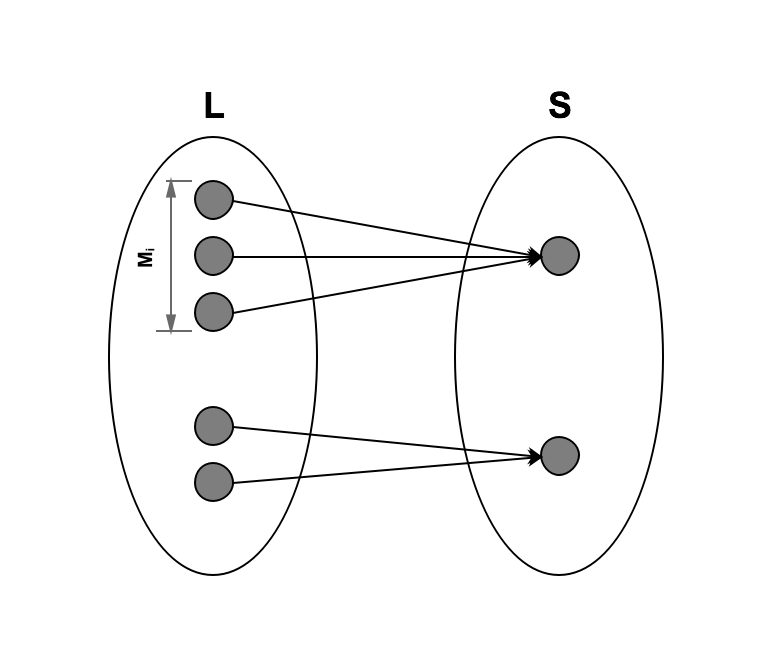
\includegraphics[width=.7\linewidth]{image/falsefork.png}
\caption{ False Fork}
\end{figurehere}
\end{center}

As shown,$L$  is a collection of all possible forked accounts for a set of transactions, and $S$ is a collection of states that can be reached in different orders. According to definition ,\ref{def:fork}, mapping $f: L \rightarrow S$  is a surjective;And according to definition \ref{def:falsefork}, this mapping is not a injective. Here we calculate the probability of the false fork:

Suppose that $C$ users have the right to produce ledgers, $M = \vert L \vert$,$N = \vert S \vert$,$M_{i} = \vert L_{i} \vert$, where $L_{i} = \lbrace l \vert f(l) = s_{i}, s_{i} \in S \rbrace$.
The probability of false fork is as follows:
\begin{equation}
P_{ff} = \sum_{i=1}^{N}\left ( \frac{M_{i}}{M} \right )^{C} - \frac{1}{M^{C-1}}
\end{equation}

From this formula, we can see that in order to reduce the probability of false fork, there are two ways:
\begin{itemize}
	\item 	Establish equivalence relations on the $L$ of the ledger set, divide equivalence classes into them, and construct fewer forked ledgers.
	\item 	Restrict users who have the right to produce ledgers, thereby reducing $C$
\end{itemize}

The first way is the important direction in Vite design. It will be discussed in detail later. The second ways have been adopted by many algorithms. In the PoW algorithm, any user has the right to produce a block; and the PoS algorithm limits the power of the production block to those with system rights; the DPoS algorithm \cite{dpos}  limits the user with the right to produce the block to be further restricted within a group of agent nodes.
	
At present, through improved consensus algorithm, some influential projects appeared. For example, Cardano uses a PoS algorithm called Ouroboros, and literature \cite{bernardo2017ouroboros} gives a strict proof of the related characters of the algorithm; BFT-DPOS algorithm used by EOS\cite{eos}, is a variant of the DPoS algorithm and improves system throughput by fast producing blocks; Qtum \cite{dai2017smart}'s consensus algorithm is also a PoS algorithm; The Casper algorithm adopted by RChain \cite{rchain} is one of the PoS algorithms as well.

There are also other projects that put forward their own proposals for improving the consensus algorithm. NEO\cite{neo} uses a BFT algorithm, called dBFT, and Cosmos\cite{cosmos} uses an algorithm called Tendermint  \cite{tendermint}.

\section{Ledgers}
\subsection{Overview}
The role of ledgers is to determine the order of transactions, and the order of transactions will affect the following two aspects:
\begin{itemize}
	\item \textbf{Consistency of status:} Since the state of the system is not a CRDT (Conflict-free replicated data types) \cite{crdt}, not all transaction is exchangeable, and the sequence of different transaction execution may lead to the system entering a different state.
	\item \textbf{Effectiveness of Hash:} In the ledger, the transaction will be packaged into blocks, which contain hash that is referenced each other. The order of transactions affects the connectivity of hash quoted in the ledgers. The greater the scope of this impact, the greater the cost of tampering with transactions. This is because any change to a transaction must be rebuilt by hash, which directly or indirectly refers to the block of the transaction..
\end{itemize}

The design of the ledger also has two main objectives:

\begin{center}
\begin{figurehere}
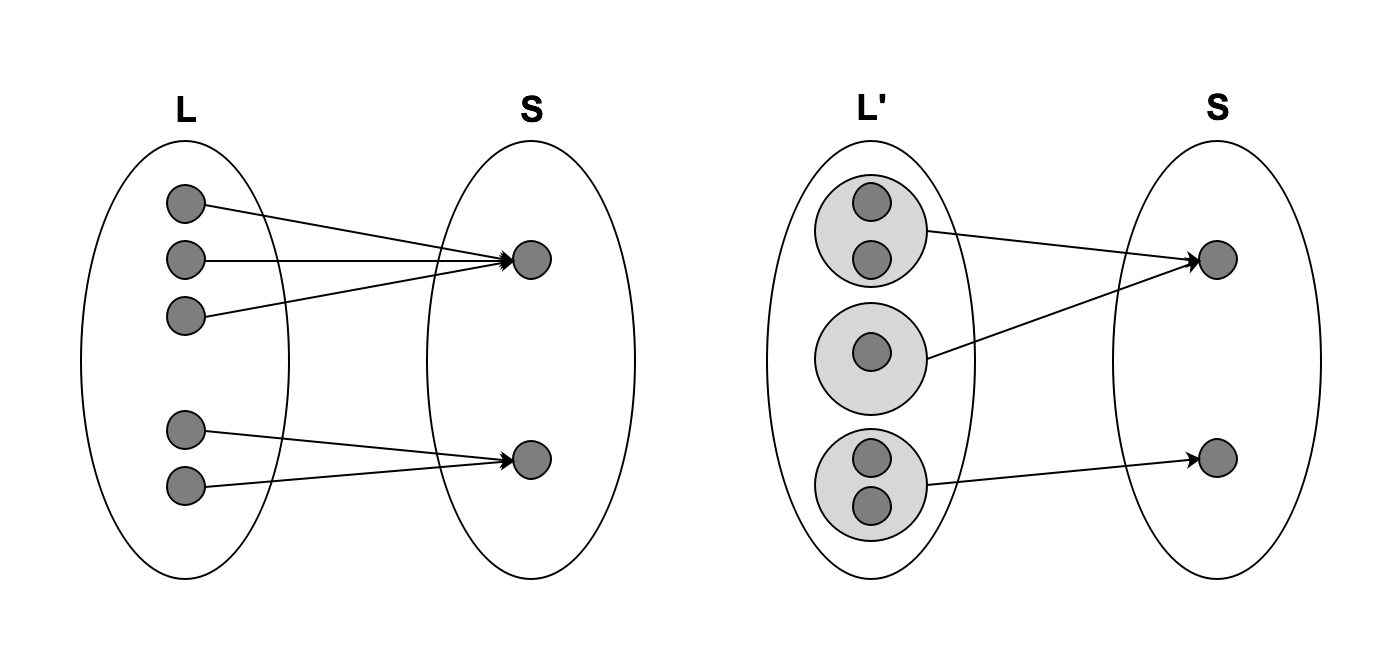
\includegraphics[width=.7\linewidth]{image/ledger-merge.png}
\caption{Ledger merge}
\end{figurehere}
\end{center}

\begin{itemize}
	\item \textbf{Reducing the false fork rate:} as discussed in the previous section, the reduction of the false fork rate can be achieved by establishing an equivalent class and combining a group of accounts that lead the system into the same state into a single account. As shown above, according to the formula of false fork rate, the false fork rate of the ledger on the left is $P_{ff}=\left (  \frac{3}{5} \right )^{C} + \left (  \frac{2}{5} \right )^{C} - \frac{1}{5^{C-1}}$;after the merge of ledger space, the false fork rate of the right graph is ${P_{ff}}'=\left (  \frac{2}{3} \right )^{C} + \left (  \frac{1}{3} \right )^{C} - \frac{1}{3^{C-1}}$.It is known that when $C > 1$,${P_{ff}}' < P_{ff}$. That is to say, we should minimize the partial ordering relationship between transactions and allow more transactions to be exchanged sequentially.
	\item \textbf{Tamper proof:} when a transaction $t$ is modified in the ledger $l$,in the two sub ledgers of the book $l = l_{1} + l_{2}$, the sub ledger  $l_{1}$ is not affected, and the hash references in the sub ledger $l_{2}$ need to be rebuilt to form a new valid ledger ${l}' = l_{1} + {l_{2}}'$. Affected sub ledger $l_{2} = \Gamma(T_{2}),T_{2} = \lbrace x \vert x \in T, x > t \rbrace $.Thus, to increase the cost of tampering with transactions, it is necessary to maintain the partial order relationship between transactions as much as possible in order to expand the scope of tampering $\vert T_{2} \vert$.
\end{itemize}

\begin{center}
\begin{figurehere}
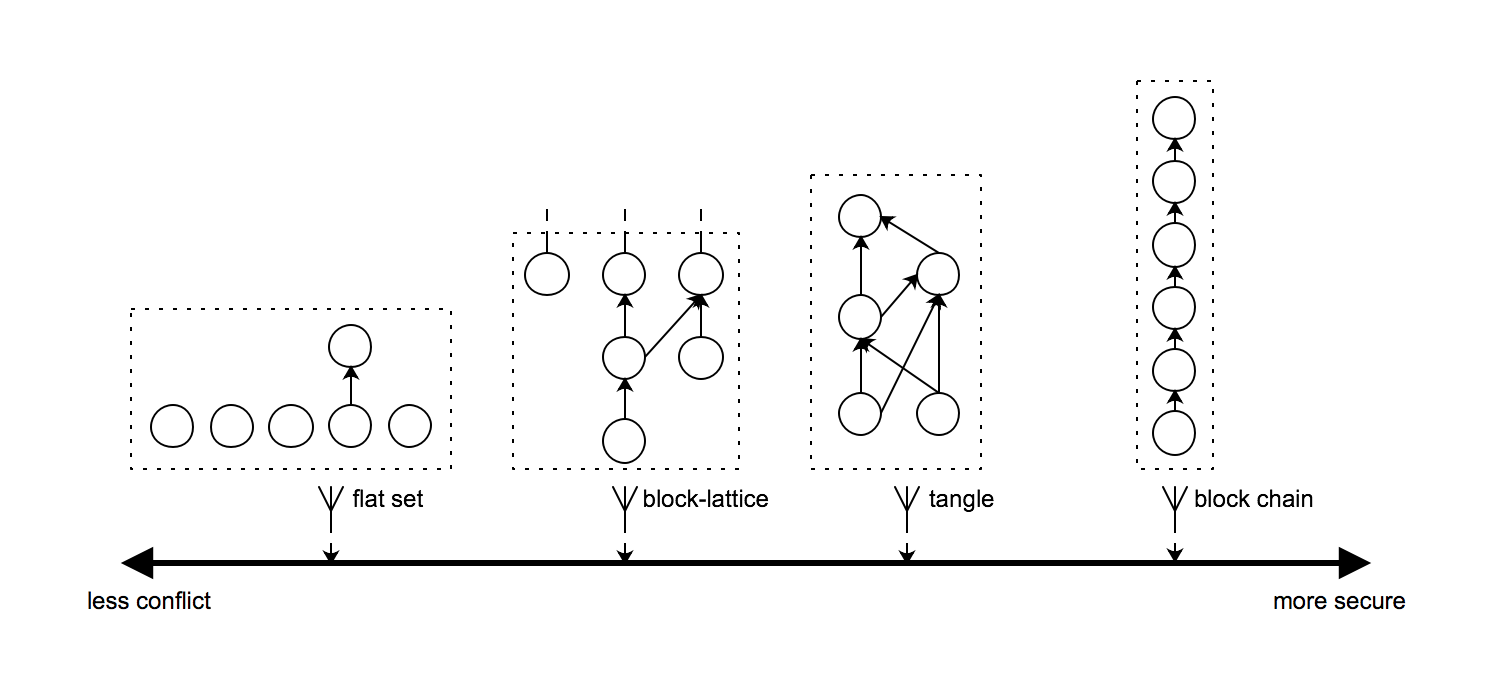
\includegraphics[width=\linewidth]{image/ledger-compare.png}
\caption{Ledger structure comparison}
\end{figurehere}
\end{center}

Obviously, the above two objectives are contradictory, and the necessary trade-offs must be made when designing the account structure. Since the account maintenance is a partial order between transactions, it is essentially a partial ordered set (poset) \cite{poset}, if represented by Hasse diagram (Hasse diagram)\cite{hasse}, it is a DAG on the topology.

The above picture compares several common ledger structures, and the ledgers near the left are maintained with less partial order. Hasse diagram appears flat and has a lower false fork rate; the ledgers near the right side maintain more partial order relationships, and Hasse diagram is more slender and more tamper resistant.

In the picture, the most-left side is a common set based structure in a centralization system without any tamper proofing features; the most right side is a typical blockchain Ledger with the best tamper proof features; between the two, there are two DAG ledgers,  the block-lattice account \cite{nano} used by Nano on the left; and the right side, the tangle book \cite{iota} is used by IOTA . In terms of characteristics, blocklattice maintains less partial order relations and is more suitable for the accounting structure of high performance decentralized application platforms. Because of its poor tampering characteristics, it can expose security risks, so far, no other projects adopt this ledger structure except Nano.

In order to pursue high performance, Vite adopts the DAG ledger structure.  At the same time, by introducing an additional chain structure Snapshot Chain and improving the consensus algorithm, the shortcomings of block-lattice security are successfully made up, and the two improvements will be discussed in detail later.

\subsection{Pre Constraint}
First, let's take a look at the precondition of using this ledger structure for the state machine model. This structure is essentially a combination of the entire state machine as a set of independent state machines, each account corresponding to an independent state machine, and each transaction only affects the state of an account. In the ledger, all transactions are grouped into accounts and organized into a chain of transactions in the same account. Therefore, we have the following restrictions on the state S and transaction T in Vite:

\begin{definition}[Single degree of freedom constraint]
system state $s \in S$,is the vector $s=(s_{1}, s_{2},...,s_{n})$ formed by the state $s_{i}$ of each account. For $\forall t_{i} \in T$,after performing the transaction $t_{i}$, the system state transfers as follows: $({s_{1}}',..., {s_{i}}',...,{s_{n}}') = \sigma(t_{i}, (s_{1},..., s_{i},...,s_{n}))$,need to meet:${s_{j}}'=s_{j} , j \neq i$.This constraint is called a single degree of freedom constraint for a transaction.
\end{definition}

Intuitively, a single degree of freedom transaction will only change the state of an account without affecting the status of other accounts in the system. In the multidimensional space where the state space vector is located, a transaction is executed, and the state of the system moves only along the direction parallel to a coordinate axis. Please note that this definition is more stringent than the transaction definition in Bitcoin, Ethereum and other models. A transaction in Bitcoin will change the state of the two accounts of the sender and the recipient; the Ethereum may change the state of more than two accounts through a message call.

Under this constraint, the relationship between transactions can be simplified. Any two transaction is either orthogonal or parallel. This provides conditions for grouping transactions according to accounts. Here is an example to illustrate:

\begin{center}
\begin{figurehere}
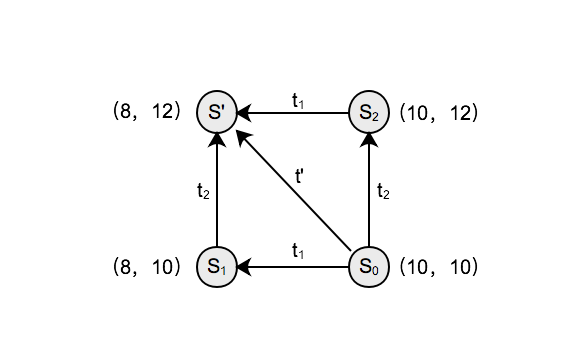
\includegraphics[width=.8\linewidth]{image/tx-deg-of-free.png}
\caption{Single degree of freedom trading and intermediate state}
\end{figurehere}
\end{center}

As shown in the figure above, suppose Alice and Bob  have 10 USD respectively. The initial state of the system is $s_{0} = (10, 10)$. When Alice wants to transfer 2 USD to Bob, in the model of  Bitcoin and Ethereum, a transaction${t}'$,can make the system go directly into the final state:$s_{0} \overset{{t}'}{\rightarrow}{s}'$.

In the definition of Vite, transaction ${t}'$ changed the status of two accounts of Alice and Bob as well, which did not conform to the principle of single degree of freedom. Therefore, the transaction must be split into two transactions:

1) A transaction $t_{1}$ that represents transferring of 2 USD by Alice

2) A transaction $t_{2}$ that represents receiving of 2 USD by Bob 

In this way, from the initial state to the final state ${s}'$ there could be two different paths $s_{0} \overset{t_{1}}{\rightarrow} s_{1} \overset{t_{2}}{\rightarrow} {s}'$ and $s_{0} \overset{t_{2}}{\rightarrow} s_{2} \overset{t_{1}}{\rightarrow} {s}'$. These two paths are respectively passed through the intermediate state $s_{1}$ and $s_{2}$, and these two intermediate states are the mapping of the final state ${s}'$ in the two account dimensions.In other words, if you only care about the state of one of the accounts, you only need to execute all the transactions that correspond to the account, and do not need to carry out the transactions of other accounts.

Next, we will define how to split transactions in Ethereum into the single degree of freedom transactions required by Vite:
\begin{definition}[Transaction Decomposition]
Dividing a transaction with a degree of freedom greater than 1 into a set of single degree of freedom transactions, named Transaction Decomposition. A transfer transaction can be split into a sending transaction and a receiving transaction; a contract call transaction can be split into a contract request transaction and a contract response transaction; a message call within each contract can be split into a contract request transaction and a contractual response transaction.
\end{definition}

Thus, there would be two different types of transactions in the ledgers. They are called "trading pairs":
\begin{definition}[Trading Pair]
a sending transaction or contract request transaction, collectively referred to as a "request transaction"; a receiving transaction or a contract response transaction, collectively referred to as "response transaction". A request transaction and a corresponding response transaction are called transaction pairs. The account for initiating the request for transaction $t$  is recorded as  $A(t)$; the corresponding response transaction is recorded as: $\widetilde{t}$, the account corresponding to the transaction is recorded as  $A(\widetilde{t})$.
\end{definition}

Based on the above definition, we can conclude the possible relationship between any two transactions in Vite:
\begin{definition}[Transaction Relationship]
There may exist for the following relations for two transactions $t_{1}$ and $t_{2}$:

\textbf{Orthogonality}:If $A(t_{1}) \neq A(t_{2})$,the two transactions are orthogonal , recorded as$t_{1} \perp t_{2}$;

\textbf{Parallel}:If $A(t_{1}) = A(t_{2})$,the two transactions are parallel, recorded as $t_{1} \parallel t_{2}$;

\textbf{Causality}:If $t_{2} = \widetilde{t_{1}}$,then the two transactions are causal,recorded as $t_{1} \rhd t_{2}$, or $t_{2} \lhd t_{1}$.
\end{definition}

\subsection{Definition of Ledger}
To define a ledger is to define a poset. First, let’s define the partial ordering relationship between transactions in Vite:
\begin{definition}[Partial order of transactions]
we use dualistic relationship  $<$ to represent the partial order relation of two transactions:

A response transaction must follow a corresponding request transaction :$t_{1} < t_{2} \Leftrightarrow t_{1} \rhd t_{2}$;

All transactions in an account must be strictly and globally ordered:$\forall t_{1} \parallel t_{2}$, there must be :$t_{1} < t_{2}$,or $t_{2} < t_{1}$.
\end{definition}

Due to the partial ordering relationship established on the transaction set $T$ meet the characteristics:
\begin{itemize}
	\item Irreflexive: $\forall t \in T$,there is no $t < t$;
	\item Transitive:$\forall t_{1},t_{2},t_{3} \in T$, if $t_{1}<t_{2},t_{2}<t_{3}$, then $t_{1}<t_{3}$;
	\item Asymmetric:$\forall t_{1},t_{2} \in T$, if $t_{1}<t_{2}$, then it doesn't exist $t_{2}<t_{1}$
\end{itemize}

In this way, we can define the Vite account in strict partial order set:

\begin{definition}[Vite Ledger]
Vite Ledger is thestrict poset composed by set of $T$ of the given transaction, and the partial poset $<$ 
\end{definition}

\begin{center}
\begin{figurehere}
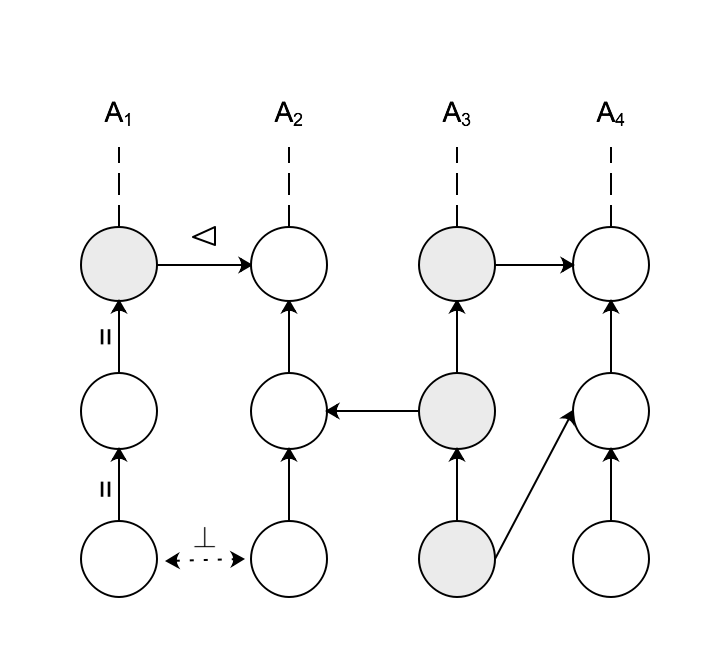
\includegraphics[width=.7\linewidth]{image/ledger.png}
\caption{The relationship between the ledger and the transaction in Vite}
\end{figurehere}
\end{center}

A strict poset can correspond to a DAG structure. As shown in the figure above, circles represent transactions, and arrows denote dependencies between transactions. $a \rightarrow b$ indicates that $a$ depends on $b$.

The Vite ledger defined above is structurally similar to block-lattice. Transactions are divided into request and response transactions, each of which corresponds to a separate block, each account Ai corresponds to a chain, a transaction pair, and a response transaction referencing the hash of its corresponding request transaction.


\section{Snapshot chain}
\subsection{Transaction Confirmation}
When the account is forked, the result of consensus may swing between two forked ledgers. For example, based on a blockchain structure, if a node receives a longer forked chain, the new fork will be selected as the consensus result, and the original fork will be abandoned and the transaction on the original fork will be rolled back. In such a system, transaction rollback is a very serious event, which will lead to double spend. Just imagine that a business receives a payment, provides goods or services, and after that payment is withdrawn, the merchant may face losses. Therefore, when a user receives a payment transaction, it needs to wait for the system to "confirm" the transaction to ensure that the probability of rolling back is low enough.

\begin{definition}[Transaction Confirmation]
when the probability of a transaction being rolled back is less than a given threshold $\epsilon$, the transaction is called confirmed.
$P_{r}(t) < \epsilon \Leftrightarrow t \text{ is } \boldsymbol{confirmed}$.
\end{definition}

Confirmation of transactions is a very confusing concept, because whether a transaction is recognized depends in fact on the implicit confidence level of $1-\epsilon$. A merchant selling diamonds and a coffee seller suffered different losses when they were attacked by double spend. As a result, the former needs to set smaller $\epsilon$ on the transaction. This is also the essence of the number of confirmations in Bitcoin. In Bitcoin, the confirmation number indicates the depth of a transaction in the block chain. The greater the number of confirmations, the lower the probability of the transaction being rolled back \cite{nakamoto2008bitcoin}. Therefore, merchants can indirectly set the confidence level of the confirmation by setting the waiting number of confirmation numbers.

The probability of transaction rollback decreases with time due to the hash reference relationship in the account structure. As mentioned above, when the design of the ledger has better tampering characteristics, rolling back a transaction needs to reconstruct all subsequent blocks of the exchange in the block. As new transactions are constantly being added to ledgers, there are more and more successive nodes in a transaction, so the probability of being tampered with will decrease. 

In the block-lattice structure, as the transaction is grouped by account, a transaction will only be attached to the end of the account chain of its own account, and the transaction generated by most other accounts will not automatically become a successor node of the transaction. Therefore, it is necessary to design a consensus algorithm reasonably to avoid hidden dangers of double spend.

Nano adopts a voting based consensus algorithm, \cite{nano}, transaction is signed by a set of representative nodes selected by a group of users. Each representative node has a weight. When the signature of a transaction has enough weight, it is believed that the transaction is confirmed. There are following problems in this algorithm:

First, if a higher confidence degree of confirmation is needed, the threshold of the voting weight needs to be raised. If there are not enough representative nodes online, the intersecting speed can not be guaranteed, and it is possible that a user will never collect the number of tickets necessary to confirm an exchange;

Second, the probability that transactions are rolled back does not decrease with time. This is because at any time, the cost of overthrowing a historical voting is the same.

Finally, the historical voting results are not persisted into the ledger, and are stored only in the local storage of nodes. When a node gets its account from other nodes, there is no way to reliably quantify the probability of a historical transaction being rolled back.

In essence, the voting mechanism is a partial centralization solution. We can regard the voting results as a snapshot of the status of the ledgers. This snapshot will be distributed in the local storage of each node in the network. In order to have the same tamper proof ability with the block chain, we can also organize these snapshots into chain structures, which is one of the kernel of the Vite design - the snapshot chain \cite{snapshotchain}.

\subsection{Definition of snapshot chain}
Snapshot chain is the most important storage structure in Vite. Its main function is to maintain the consensus of Vite ledgers. First, we give the definition of the snapshot chain: 
\begin{definition}[Snapshot block and snapshot chain]
a snapshot block that stores a state snapshot of a Vite ledger, including the balance of the account, the Merkle root of the contract state, and the hash of the last block in each account chain. The snapshot chain is a chain structure composed of snapshot blocks, and the next snapshot block refers to the hash of the previous snapshot block.
\end{definition}

The state of a user account contains the balance and the hash of the last block of the account chain; in addition to the above two fields, the state of a contract account contains the Merkle root hash of it, The structure of the state of an account is as follows:

\begin{verbatim}
  struct AccountState {
    // account balance
    map<uint32, uint256> balances;
    // Merkle root of the contract state
    optional uint256 storageRoot;
    // hash of the last transaction
    // of the account chain
    uint256 lastTransaction;
  }
\end{verbatim}

The structure of the snapshot block is defined as follows:
\begin{verbatim}
  struct SnapshotBlock {
    // hash of the previous block   
    uint256 prevHash;
    // snapshot information
    map<address, AccountState> snapshot;
    // signature
    uint256 signature;
  }
\end{verbatim}

In order to support multiple tokens at the same time, the structure of recording the balance information in Vite's account state is not a \texttt{uint256}, but a mapping from the token ID to the balance.

The first snapshot block in the snapshot chain is called the "genesis snapshot", which saves snapshots of the genesis block in the account.

\begin{center}
\begin{figurehere}
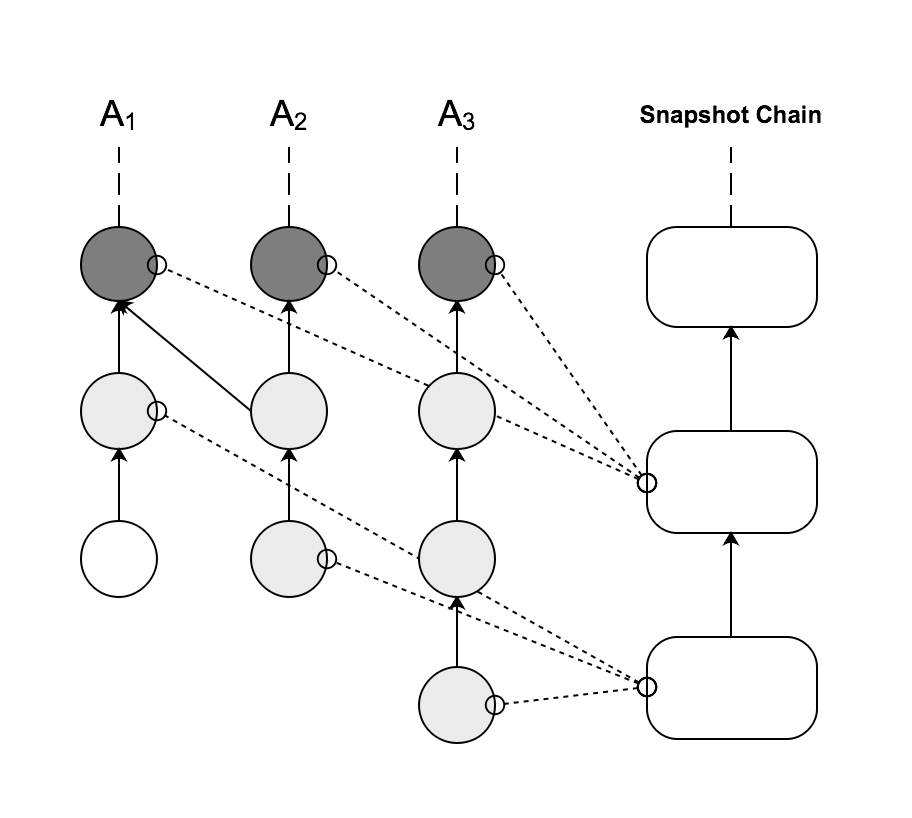
\includegraphics[width=.7\linewidth]{image/snapshotchain.png}
\caption{snapshot chain}
\end{figurehere}
\end{center}

Since each snapshot block in the snapshot chain corresponds to the only fork of the Vite ledger, it is possible to determine the consensus result of the Vite ledger by the snapshot block when the snapshot block does not fork in the snapshot block.

\subsection{Snapshot chain and transaction confirmation}

After introducing the snapshot chain, the natural security flaws of block-lattice structure have been remedied. If an attacker wants to generate a double spend transaction, in addition to rebuilding the hash reference in the Vite ledger, it also needs to be rebuilt in the snapshot chain for all the blocks after the first snapshot block of the transaction, and need to produce a longer snapshot chain. In this way, the cost of attack will be greatly increased.

In Vite, the confirmation mechanism of transactions is similar to Bitcoin, which is defined as follows:

\begin{definition}[Transaction Confirmation in Vite]
 in Vite,if a transaction is snapshot by snapshot chain, the transaction is confirmed., the depth of the snapshot block in the first snapshot, is called the confirmation number of the transaction.
\end{definition}

Under this definition, the number of confirmed transactions will increase by 1 when the snapshot chain grows, and the probability of the double spend attack decreases with the increase of the snapshot chain. In this way, users can customize the required confirmation number by waiting for different confirmation numbers according to the specific scenario.

The snapshot chain itself relies on a consensus algorithm. If the snapshot chain is forked, the \textbf {longest} fork is chosen as a valid fork. When the snapshot chain is switched to a new fork, the original snapshot information will be rolled back, that means the original consensus on the ledger was overthrown, and replaced by the new consensus. Therefore, snapshot chain is the cornerstone of the whole system security, and needs to be treated seriously.

\subsection{Compressed storage}
Because all account states need to be saved in every snapshot block in snapshot chain, the storage space is to be very large, the compression to the snapshot chains is necessary.

\begin{center}
\begin{figurehere}
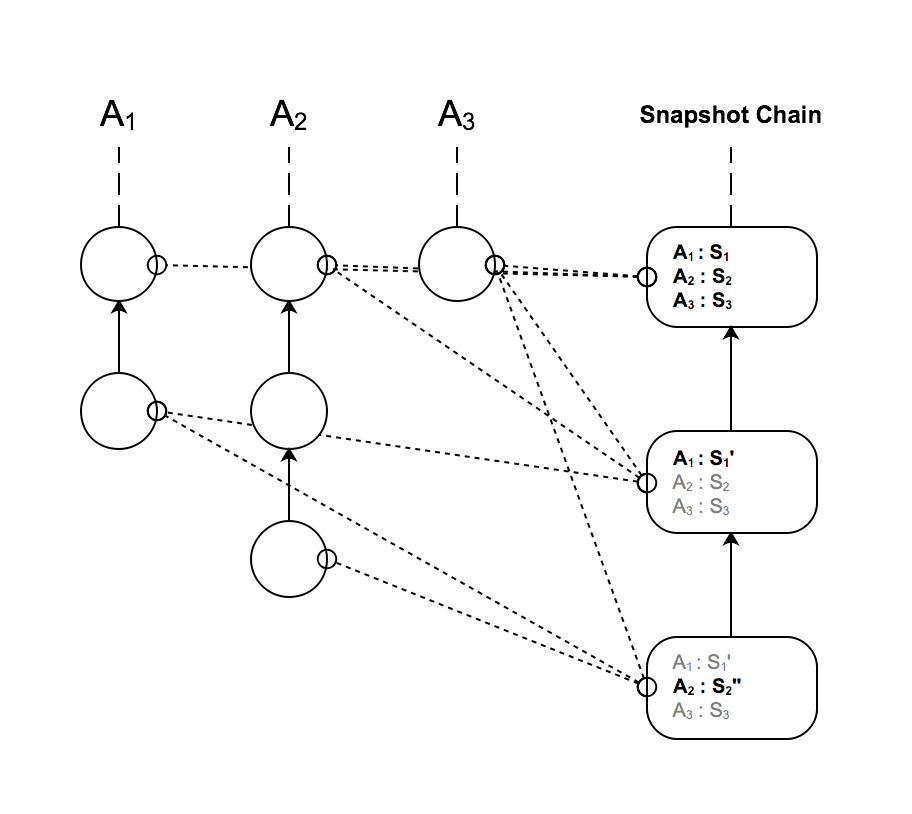
\includegraphics[width=.7\linewidth]{image/compact-snapshot.png}
\caption{Snapshot before compression}
\end{figurehere}
\end{center}

The basic approach of compressing snapshot chain storage space is to use incremental storage: a snapshot block only stores data that is changed compared to the previous snapshot block. If there is no transaction for one account between the two snapshots, the latter snapshot block will not save the data of the account.

To recover snapshot information, you can traverse the snapshot block from the beginning to the end, and cover the data of every snapshot block by the current data.

\begin{center}
\begin{figurehere}
\centering
\tikzstyle{block} = [draw, fill=blue!20, rectangle, 
    minimum height=3em, minimum width=6em]
\tikzstyle{sum} = [draw, fill=blue!20, circle, node distance=1cm]
\tikzstyle{input} = [coordinate]
\tikzstyle{output} = [coordinate]
\tikzstyle{pinstyle} = [pin edge={to-,thin,black}]

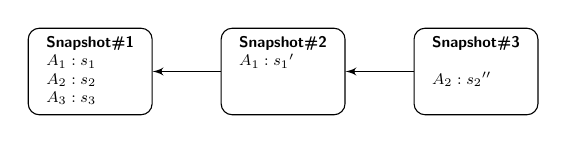
\begin{tikzpicture}[
    auto, 
    node distance=2cm,
    >=latex',
    font=\bfseries\footnotesize\sffamily,
    snapshot/.style={
		scale=0.7,
		rectangle,
		rounded corners,
		draw=black, 
		text centered,
%		text width=5cm,
		minimum height=12mm,
		fill=white
	},
	label/.style={
		scale=0.7
	}
  ]
    % We start by placing the blocks

  \node [snapshot] (snapshot2) 
 {%
 \begin{tabular}{l}
  \textbf{Snapshot\#2}\\
  $A_{1}: {s_{1}}'$\\
  \\
  \\
 \end{tabular}
 };
 
  \node [snapshot, xshift=-3.5cm] (snapshot1) 
 {%
 \begin{tabular}{l}
  \textbf{Snapshot\#1}\\
  $A_{1}: s_{1}$\\
  $A_{2}: s_{2}$\\
  $A_{3}: s_{3}$
 \end{tabular}
 };
 
 
  \node [snapshot, xshift=3.5cm] (snapshot3) 
 {%
 \begin{tabular}{l}
  \textbf{Snapshot\#3}\\
  \\
  $A_{2}: {s_{2}}''$\\
  \\
 \end{tabular}
 };
 
 \draw [draw,->] (snapshot2) -- (snapshot1);
 \draw [draw,->] (snapshot3) -- (snapshot2);

\end{tikzpicture}

\caption{Snapshot after compression}
\label{fig:compact-snapshot}
\end{figurehere}
\end{center}

Only the final status of each snapshot of an account is saved when snapshotting, the intermediate state will not be taken into account, so only one copy of the data in the snapshot will be saved, no matter how many transactions generated by an account between the two snapshots. Therefore, a snapshot block takes up to $S * A$ bytes in maximum. Among them, $S = \text{sizeof}(s_{i})$, is the number of bytes occupied for each account state, and $A$ is the total number of system accounts. If the average ratio of active accounts to total accounts is $a$, the compression rate is $1-a$.

\section{Consensus}
\subsection{Goal of Design}
When designing a consensus protocol, we need to take full account of the following factors:
\begin{itemize}
	\item \textbf{Performance}.The primary goal of Vite is fast. To ensure high throughput and low delay performance of the system, we need to adopt a consensus algorithm with higher convergence speed.
	\item \textbf{Scalability}.Vite is a public platform that is open to all decentralized applications, so Scalability is also an important consideration.
	\item \textbf{Security}.The design principle of Vite is not pursuing the ultimate safety, however, it still needs to ensure enough safety base line and effectively guard against all kinds of attacks.
\end{itemize}

Compared with some existing consensus algorithms, the security of PoW is better, and a consensus can be reached if the computing power of malicious nodes are below 50\%. However, the intersecting speed of PoW is slow and can not meet the performance requirements; PoS and its variant algorithms remove the steps to solve mathematical problems, improve intersecting speed and single attack cost, and reduce energy consumption. But the Scalability of PoS is still poor, and the “Nothing at Stake” problem \cite{problems} is difficult to solve; BFT algorithms has better performance in security and performance, but its Scalability is a problem, usually more suitable for private chain or consortium chain; the DPoS \cite{dpos} series algorithm effectively reduces the probability of false fork by limiting the permissions of generating blocks. The performance and scalability are good. As a consequence, DPoS has a slight sacrifice in security, and the number of malicious nodes should not be more than 1/3 \cite{dpos2}.

Generally, the DPoS algorithm has obvious advantages in performance and scalability. Therefore, we choose DPoS as the basis of the Vite consensus protocol and expand it properly on the basis of it. Through Hierarchical Delegated consensus protocol and asynchronous model, the overall performance of the platform can be further improved.

\subsection{Hierarchical Consensus}
The consensus protocol of Vite is HDPoS (Hierarchical Delegated Proof of Stake). The basic idea is to decompose the consensus function $\Phi$ (functional decomposition):
\begin{equation}
\begin{split}
\Phi(l_1,l_2,\dots,l_n) = \Psi(\Lambda_1(l_1,l_2,\dots,l_n), \\
\Lambda_2(l_1,l_2,\dots,l_n),\dots \\
\Lambda_m(l_1,l_2,\dots,l_n))
\end{split}
\end{equation}

$\Lambda_i: 2^L \rightarrow L$,is called as local consensus function,the returned result is called the local consensus; $\Psi: 2^L \rightarrow L$, known as the global consensus function, it selects a unique result from a group of candidate in local consensus as the final consensus result.

After this separation, the consensus of the whole system has become two independent processes:
\begin{labeling}{alligator}
\item [Local consensus] generate the blocks corresponding to request transactions and response transaction in the user account or contract account, and writes to the ledgers.
\item [Global consensus] snapshots the data in the ledger and generates snapshot blocks. If the ledger is forked, choose one of them.
\end{labeling}

\subsection{Right of Block Generation and Consensus Group}
Then, who has the right to generate the transaction block in the ledger and snapshot block in the snapshot chain? What consensus algorithm is adopted to reach a consensus?
Since the ledger structure of Vite is organized into multiple account chains according to different accounts, we can conveniently define both the right of production of the blocks in the ledger according to the dimension of the account, and the production right of the snapshot block belong to to a single group of users. In this way, we can put a number of account chains or snapshot chains into a consensus group, and in the consensus group, we can use a unified way to produce the block and reach a consensus.

\begin{definition}[Consensus Group]
Consensus group is a tuple $(L, U, \Phi, P)$, describing the consensus mechanism of a portion of the account or snapshot chain.,$L \in A \vert \{ A_s \}$,  represents one or a number of account chains, or snapshot chains of the consensus group in the ledger; $U$ represents the user with the block production right on the chain specified by the $L$; $\Phi$ specifies the consensus algorithm of the consensus group; and $P$ specifies the parameters of the consensus algorithm.

\end{definition}

Under this definition, users can set up consensus groups flexibly and select different consensus parameters on their needs. Next, we will elaborate on different consensus groups.

\subsubsection{Consensus Group of Snapshot}
The consensus group of snapshot chains is called snapshot consensus group, which is the most important consensus group in Vite. The consensus algorithm $\Phi$ of snapshot consensus group adopts the DPoS algorithm and corresponding to $\Psi$ in the hierarchical model. The number of agents and the interval of the block generation are specified by the parameter $P$.

For example, we can specify snapshot consensus groups with 25 proxy nodes to produce snapshot blocks at intervals of 1 second. This ensures that the transaction is confirmed to be fast enough. Achieving 10 times transaction confirmation need to wait 10 seconds in maximum.

\subsubsection{Private Consensus Group}
The private consensus group is only applicable to the production of transaction blocks in ledgers, and belongs to the account chain of private consensus group. The blocks can only be produced by the owner of the private key of the account. By default, all user accounts belong to the private consensus group. 

The greatest advantage of the private consensus group is to reduce the probability of fork. Because only one user has the right to produce blocks, the only possibility of fork is that the user initiate a double spend attack personally or a program error.

The disadvantage of the private consensus group is that the user nodes must be online before they can pack the transaction. This is not very suitable for the contract account. Once the owner's node fails, no other node can replace the response transaction that it produces contracts, which is equivalent to reducing the service availability of dApp.

\subsubsection{Delegate Consensus Group}
In the delegate consensus group, instead of user account ,a set of designated proxy nodes is used to package the transaction through the DPoS algorithm. Both user accounts and contractual accounts can be added to the consensus group. Users can set up a set of separate agent nodes and establish a new consensus group. There is also a default consensus group in Vite to help package transactions for all the other accounts that haven’t established their delegate consensus group individually, which is also known as the \textbf {public consensus group}.

The delegate consensus group is suitable for most of the contract accounts, because most of the transactions in the contract account are contract response transactions, in which higher availability and lower delays are needed than the receivable transactions in the user account.

\subsection{The Priority of the Consensus}\label{sec:consensus-prio}
In the Vite protocol, the priority of global consensus is higher than that of local consensus. When the local consensus is forked, the result of global consensus selection will prevail. In other words, once the global consensus selected a fork of the local consensus as the final result, even a longer fork of a certain account chain in the future accounts occurs, it will not cause the roll back of the global consensus results.

This problem needs more attention when implementing cross chain protocol. Because a target chain may roll back, the corresponding account chain of the relay contract mapping the chain also needs to roll back accordingly. At this moment, if the local consensus of the relay chain has been adopted by the global consensus, it is impossible to complete the rollback, which may cause the data between the relay contract and the target chain to be inconsistent.

The way to avoid this problem is to set a parameter \textit{delay}  in the consensus group parameter $P$, which specifies the snapshot consensus group to take a snapshot only the local consensus is completed after \textit{delay} blocks. This will greatly reduce the probability of inconsistency of relay contracts, but it can’t be avoided completely. In the code logic of relay contracts, it is also necessary to deal with the rollback of the target chain separately.

\subsection{Asynchronous Model}
In order to improve system throughput further, we need to support a more perfect asynchronous model on the consensus mechanism.

The life cycle of a transaction includes transaction initiation, transaction writing and transaction confirmation. In order to improve the performance of the system, we need to design these three steps into asynchronous mode. This is because at different times, the quantity of transactions initiated by users is different, the speed of transaction writing and transaction confirmation processed by system is fixed relatively. Asynchronous mode helps to flatten the peaks and troughs thus improve the overall throughput of the system. 

The asynchronous model of the Bitcoin and the Ethereum is simple: the transaction initiated by all users is placed in an unconfirmed pool. When the miner packages it into a block, the transaction is written and confirmed at the same time. When the block chain continues to grow, the transaction eventually reaches the preset confirmation confidence level.

There are two problems in this asynchronous model:
\begin{itemize}
	\item 	Transactions are not persisted to ledgers in an unconfirmed state. Unrecognized transactions are unstable, and there is no consensus involved, it can’t prevent sending of transactions repeatedly.
	\item 	There is no asynchronous mechanism for writing and confirming of transactions. Transactions are only written when confirmed, and the speed of writing is restricted by the confirmation speed.
\end{itemize}

The Vite protocol establishes a more improved asynchronous model: first, the transaction is split into a transaction pair based on a "request - response" model, whether it is a transfer or a contract call, and the transaction is successfully launched when a request transaction is written to the ledger. In addition, the  written and confirming of a transaction is asynchronous as well. Transactions can be written into the DAG account of Vite firstly and will not be blocked by the confirmation process. Transaction confirmation is done through snapshot chain, and snapshot action is asynchronous too.

This is a typical producer - consumer model. In the life cycle of the transaction, no matter how production rate changes in the upstream, the downstream can deal with the transaction at a constant rate, so as to fully utilized the platform resources and improve the system's throughput.

\section{Virtual Machine}
\subsection{EVM compatibility}
At present, there are many developers in the Ethereum field, and many smart contracts are applied based on Solidity and EVM. Therefore, we decided to provide EVM compatibility on the Vite virtual machine, and the original semantics in most of the EVM instruction sets is kept in Vite. Because Vite's account structure and transaction definition is different from Ethereum, the semantics of some EVM instructions need to be redefined, for example, a set of instructions to get block information. The detailed semantic differences can be referred to appendix \ref{app:evm-instruction-set}..

Among them, the biggest difference is the semantics of message calls. Next we will discuss in detail.

\subsection{Event Driven}
In the protocol of Ethereum, a transaction or message may affect the status of multiple accounts. For example, a contract invocation transaction may cause the status of multiple contract accounts to change at the same time through message calls. These changes occur either at the same time, or none at all. Therefore, the transaction in the Ethereum is actually a kind of rigid transaction that satisfies the characteristics of ACID (Atomicity, Consistency, Isolation, Durability) \cite{Haerder:1983:PTD:289.291}, which is also an important reason for the lack of expansibility in the Ethereum.

Based on considerations of scalability and performance, Vite adopted a final consistency scheme satisfying BASE (Basically Available, Soft state, Eventual consistency) \cite{Pritchett:2008:BAA:1394127.1394128} semantics. Specifically, we design Vite as an Event-Driven Architecture (EDA) \cite{eda}. Each smart contract is considered to be an independent service, and messages can be communicated between contracts, but no state is shared.

Therefore, in the EVM of Vite, we need to cancel the semantics of synchronous function calls across contracts, and only allow message communication between contracts. The EVM instructions affected are mainly \textbf{CALL} and \textbf{STATICCALL}.In Vite EVM, these two instructions can’t be executed immediately, nor can they return the result of the call. They only generate a request transaction to write to the ledger. Therefore in Vite, the semantics of function calls will not be included in this instruction, but rather sends messages to an account.

\subsection{Smart Contract Language}
Ethereum provides a Turing complete programming language Solidity for developing smart contracts. To support asynchronous semantics, we extended Solidity and defined a set of syntax for message communication. The extended Solidity is called Solidity++.

Most of the syntax of Solidity are supported by Solidity++, but not including the function calls outside the contract. The developer can define messages through the keyword \emph{message} and define the message processor (MessageHandler) through the keyword \emph{on} to implement the cross - contract communication function.

For example, the contract A needs to call the add () method in contract B to update its state based on the return value. In Solidity, it can be implemented by function call. The code is as follows:

\begin{verbatim}
pragma solidity ^0.4.0;

contract B {
    function add(uint a, uint b) returns
    (uint ret) { 
        return a + b;
    }
}

contract A {
    uint total;    
   
    function invoker(address addr, uint a,
    uint b) {
        // message call to A.add()
        uint sum = B(addr).add(a, b);
        // use the return value
        if (sum > 10) {
            total += sum;
        }
    }
}
\end{verbatim}

In Solidity++, the function call code\texttt{uint sum = B(addr).add(a, b);} is no longer valid; instead of that, contract A and contract B communicate asynchronously by sending messages to each other. The code is as follows:

\begin{verbatim}
pragma solidity++ ^0.1.0;

contract B {
    message Add(uint a, uint b);
    message Sum(uint sum);
    
    Add.on {
        // read message
        uint a = msg.data.a;
        uint b = msg.data.b;
        address sender = msg.sender;
        // do things 
        uint sum = a + b;
        // send message to return result
        send(sender, Sum(sum));
    }
}

contract A {
    uint total;    
   
    function invoker(address addr, uint a,
    uint b) {
        // message call to B
        send(addr, Add(a, b))        
        // you can do anything after sending
        // a message other than using the 
        // return value
    }
    Sum.on {
        // get return data from message
        uint sum = msg.data.sum;
        // use the return data
        if (sum > 10) {
            total += sum;
        }
    }
}
\end{verbatim}

In the first line ,code \texttt{pragma solidity++ \^0.1.0;} indicates that the source code is written in Solidity++ but will not be compiled directly with the Solidity compiler to avoid that the compiled EVM code does not conform to the expected semantics. Vite will provide a specialized compiler for compiling Solidity++. This compiler is partially forward compatible: if there is no Solidity code that conflict with the Vite semantics, it can be compiled directly, otherwise the error will be reported. For example, the syntax of local function calls, transfers to other accounts will remain compatible; obtaining the return value of the cross contract function call, as well as the monetary unit \texttt{ether}, will not be compiled.

In contract A, when the \texttt{invoker} function is called, the \texttt{Add} message will be sent to the contract B, which is asynchronous and the result will not be returned immediately.Therefore, it is necessary to define a message processor in A by using the keyword \texttt{on} to receive  returned result and update the state.

In contract B, the message \texttt{Add} is monitored. After processing, a \texttt{Sum} message is sent to the sender of the message \texttt{Add} to return the result.

Messages in Solidity++ will be compiled into \textbf{CALL} instructions and a request transaction will be added to the ledger. In Vite, ledgers serve as message middleware for asynchronous communication between contracts. It ensures reliable storage of messages and prevents duplication. Multiple messages sent to a contract by the same contract can guarantee FIFO (First In First Out); messages sent by different contracts to the same contract do not guarantee FIFO.

It should be noted that the events in Solidity (Event) and the messages in Solidity++ are not the same concept. Events are sent indirectly to front through the EVM log.

\subsection{Standard Library}
Developers who develop smart contracts on Ethereum  are often plagued by the lack of standard libraries in Solidity. For example, loop verification in the Loopring protocol must be performed outside the chain, one of the important reasons is that floating-point computing function is not provided in Solidity, especially the n square root [1]\cite{loopring} for the floating numbers.

In EVM, a pre deployed contract can be called by \textbf{DELEGATECALL} command to realize the function of library function. Ethereum also provides several Precompiled Contract, which is mainly a few Hash operations. But these functions are too simple to meet the complex application needs.

Therefore, we will provide a series of standard libraries in Solidity++, such as string processing, floating point operations, basic mathematical operations, containers, sorting, and so on.

Based on performance considerations, these standard libraries will be implemented in a local extension (Native Extension) way, and most of the operations are built into the Vite local code, and the function is called only through the \textbf{DELEGATECALL} instruction in the EVM code.

The standard library can be extended as needed, but because the state machine model of the whole system is deterministic, it can not provide functions like random numbers. Similar to Ethereum, we can simulate pseudo random numbers through the hash of snapshot chains.

\subsection{Gas}
There are two main functions for Gas in the Ethereum , the first one is to quantify the computing resources and storage resources consumed by EVM code execution, and the second is to ensure that the EVM code is halted. According to the computability theory, the Halting Problem on Turing machines is an incomputable problem \cite{haltingproblems}. That means, it is impossible to determine whether a smart contract can be stopped after limited execution by analyzing the EVM code.

Therefore, the gas calculation in EVM is also retained in Vite. However, there is no Gas Price concept In Vite. Users do not buy the gas for an exchange by paying the fees, but through a quota based model to obtain computing resources. The calculation of quotas will be discussed in detail later in the chapter "economic model".

\section{Economic Model}
\subsection{Native Token}
In order to quantify platform computing and storage resources and encourage nodes to run, Vite has built a native token ViteToken. The basic unit of token is \textit{vite}, the smallest unit is \textit{attov},,$1 \: vite = 10^{18} \: attov$.

The snapshot chain is the key to the security and performance of the Vite platform. In order to incite node to participate in the transaction verification, the Vite protocol sets up the forging reward for the production of the snapshot block. Forging incentives will increase the liquidity of ViteToken and dilute the benefits of \textit{vite} holders. Therefore, we will limit inflation to 3\% per year.

On the contrary, when users issue new tokens, deploy contracts, register VNS domain names \footnote{refer to  \textit{\ref{sec:vns} naming service}} and obtain resource quotas, they need to consume or mortgage ViteToken to reduce the liquidity.

Under the combined action of these two factors, the liquidity of \textit{vite} can be maintained at a healthy level, and at the same time, it is conducive to optimizing the allocation of system resources.

\subsection{Resource Allocation}
Since Vite is a common dApp platform, the capabilities of smart contracts deployed on them vary, and each different smart contract has different requirements for throughput and delay. Even for the same smart contract, performance requirements at different stages are different.

In the design of the Ethereum , each transaction needs to be assigned a gas price when launching, so as to compete with other transactions to write accounts. This is a typical bidding model, which can effectively control the balance between supply and demand in principle. However, user is difficult to quantify the current supply and demand situation, and can not predict the price of other competitors, therefore market failure occurs easily. Moreover, the resources competing for each bid are directed against one transaction, and there is no agreement on the rational allocation of resources according to the account dimension.

\subsubsection{Quota Calculation}
We have adopted a quota based resource allocation protocol in Vite, which allows users to obtain higher resource quotas in three ways:
\begin{itemize}
\item A PoW is calculated when the transaction is initiated;
\item Mortgage a certain amount of \textit{vite} in the account;
\item To destroy a small amount of \textit{vite} in one time.
\end{itemize}

The specific quotas can be calculated through the following formula:

\begin{equation}
Q = Q_{m} \cdot \left ( \frac{2}{1+exp\left ( -\rho \times \xi^{\top} \right )} - 1  \right )
\end{equation}

Among them, $Q_{m}$ is a constant, representing the upper limit of a single account quota, which is related to the total throughput of the system and the total number of accounts.$\xi=(\xi_{d}, \xi_{s}, \xi_{f})$ is a vector that represents the cost of a user for obtaining a resource: $\xi_{d}$ is the PoW difficulty that the user calculates when generating a transaction, $\xi_{s}$ is the \textit{vite} balance of the mortgage in the account, and $\xi_{f}$ is the one-time cost that the user is willing to pay for the increase of the quota. It should be noted that ,$\xi_{f}$ is different from the handling fee. These \textit{vite} will be destroyed directly instead of paid to the miners.

In the formula, the vector $\rho=(\rho_{d}, \rho_{s}, \rho_{f})$ represents the weight of the three way of obtaining the quota, that is, the quota obtained by the destruction of 1 \: \textit{vite} is equivalent to the mortgaged $\rho_{s} / \rho_{f}$ \: \textit{vite}.

It can be seen from this formula that if the user neither mortgages \textit{vite} nor pays the one-time cost, it is necessary to calculate a PoW, otherwise there will be no quotas to initiate a transaction, which can effectively prevent dust attacks and protect the system resources from being abused. At the same time, this formula is a Logistic function. It is relatively easy for users to get lower quotas, thereby reducing the threshold of low frequency users; and high frequency users need to invest a lot of resources in order to obtain higher quotas. The extra costs they pay will increase the benefits of all users.

\subsubsection{Resource Quantification}
Because snapshot chain is equivalent to a global clock, we can use it to quantify the resource usage of an account accurately. In each transaction, the Hash of a snapshot block is quoted, the height of the snapshot block is took as the timestamp of the transaction. Therefore, according to the difference between the two transaction timestamps, we can judge whether the interval between the two transactions is long enough.

\begin{center}
\begin{figurehere}
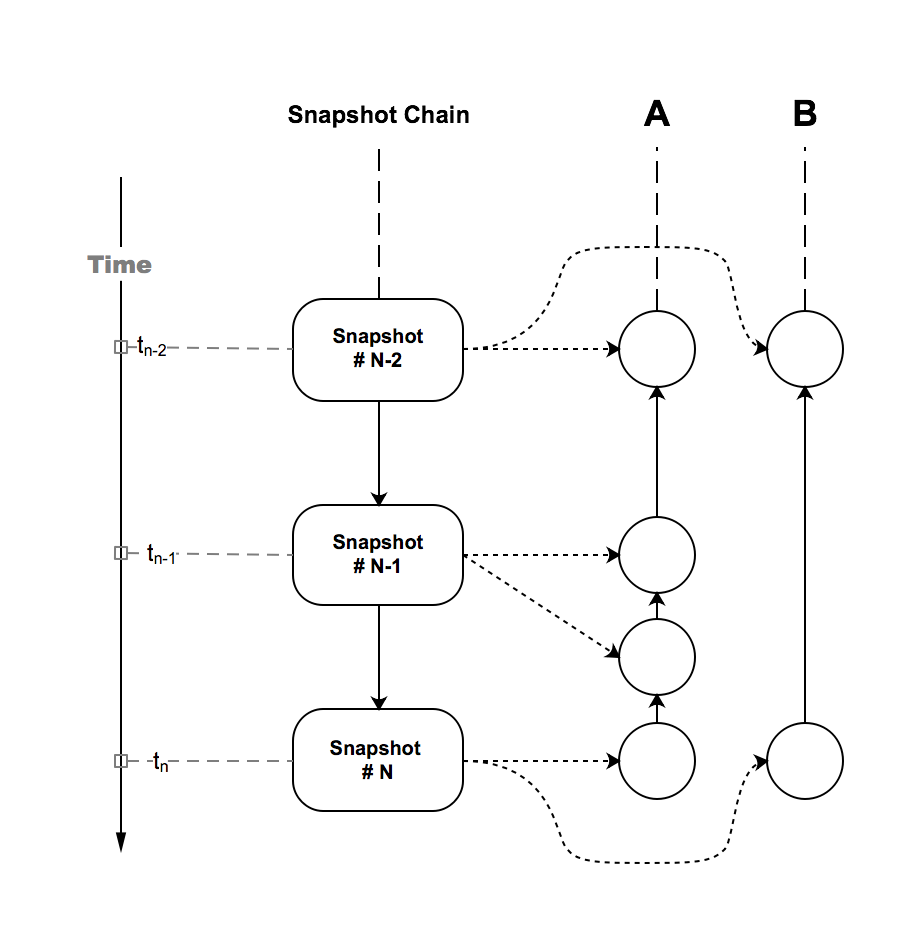
\includegraphics[width=.8\linewidth]{image/snapshotchain-clock.png}
\caption{snapshot chain as a global clock}
\end{figurehere}
\end{center}

As shown above, account $A$ generated 4 transactions in 2 time intervals, while account $B$ generated only 2 transactions. Therefore, the average TPS of  $A$ in this period is 2 times that of $B$. If it's just a transfer transaction, the average TPS of the quantified account is enough. For smart contracts, each exchange has a different consumption of resources, so it is necessary to accumulate gas for each transaction to calculate the average resource consumption for a period of time. The average resource consumption of the recent $k$ transactions in an account chain with a height of "n" is:

\begin{equation}
Cost_{k}(T_n) = \frac{k \cdot \sum_{i=n-k+1}^{n}gas_{i}}{timestamp_{n} - timestamp_{n-k+1} + 1} 
\end{equation}

Among them, for a transaction $T_n$, $timestamp_n$ is the timestamp of the transaction, that is, the height of the snapshot block it refers to; $gas_n$ is the fuel consumed for the transaction.

When verifying a transaction, the node will determine whether the quota satisfies the condition: $Cost(T) \leq Q$, and if it is not satisfied, the transaction will be rejected. In this case, users need to repackage a transaction, increase quotas by paying a one-time fee, or wait for a period of time to quote a higher snapshot in the transaction.

\subsubsection{Quota Lease}

If a user holds abundant \textit{vite} assets, but does not need to utilize so many resource quotas, he can choose to rent his quota to other users.

The Vite system supports a special type of transaction to transfer the right to use an account resource quota. In this transaction, the number of \textit{vite} that can be mortgaged, the address of a transferee, and the duration of a lease can be specified. Once the transaction is confirmed, the resource quota corresponding to the amount of the token will be included in the assignee's account. Once the lease time is exceeded, the quota will be calculated into the transferor account. The unit of leasing time is second. The system will be converted into the height difference of the snapshot block, so there may be some deviation.

The leasing income can be obtained by the user. The Vite system only provides a quota transfer transaction, and the pricing and payment of the leasing can be achieved through a third party smart contract..

\subsection{Asset Issurance}
In addition to native token ViteToken, Vite also supports users to issue their tokens. The issue of tokens can be done through a special transaction, Mint Transaction. The target address of the mint transaction is 0. In the field \textit{data} of the transaction, the parameters of the token are specified as follows:

\begin{verbatim}
Mint: {
    name: "MyToken",
   	totalSupply: 99999999900000000000000000,
   	decimals: 18,
   	owner: "0xa3c1f4...fa",
    symbol: "MYT"
}
\end{verbatim}

Once the request is accepted by the network, the \textit{vite} included in the mint transaction will be deducted from the initiator account as the mint transaction fee. The system records the information of the new token and assigns a \textit{token\_id} to it. All the balances of the newly generated tokens will be added to the \textit{owner} address, that is to say, the owner account is the genesis account of the token.

\subsection{Cross Chain Protocol}
In order to support cross chain value transmission of digital assets and eliminate "value island", Vite designed a Vite Cross-chainTransfer Protocol (VCTP).

For every asset that needs cross-chain transmission on the target chain, a token that corresponds to it is needed in the Vite as the voucher of the target Token circulating within the Vite, which is called the ToT (Token of Token). For example, if you want to transfer the \textit{ether} in the Ethereum account to Vite, you can issue a ToT with an identifier of \textit{ETH} in Vite, the initial quantity of TOT should be equal to the total quantity of \textit{ether}.

For each target chain, there is a gateway contract on Vite to maintain the mapping relationship between Vite transactions and target chain transactions. In the consensus group where the contract is located, the node responsible for generating blocks is called cross chain Relay (VCTPRelay). Cross Chain Relay needs to be the Vite node and the whole node of the target chain at the same time, and monitor transactions on both sides. On the target chain, we also need to deploy a gateway contract representing Vite.

Before cross chain relay starts to work, the corresponding ToT in Vite should be transferred to the gateway contract. After that, the supply of ToT can only be controlled by the gateway contract, and no one can be added to ensure the 1: 1 exchange ratio between the ToT and the target asset. At the same time, the assets on the target chain are controlled by the Vite gateway contract, and no user can use it, so as to ensure that ToT has a full acceptance reserve.

\begin{center}
\begin{figurehere}
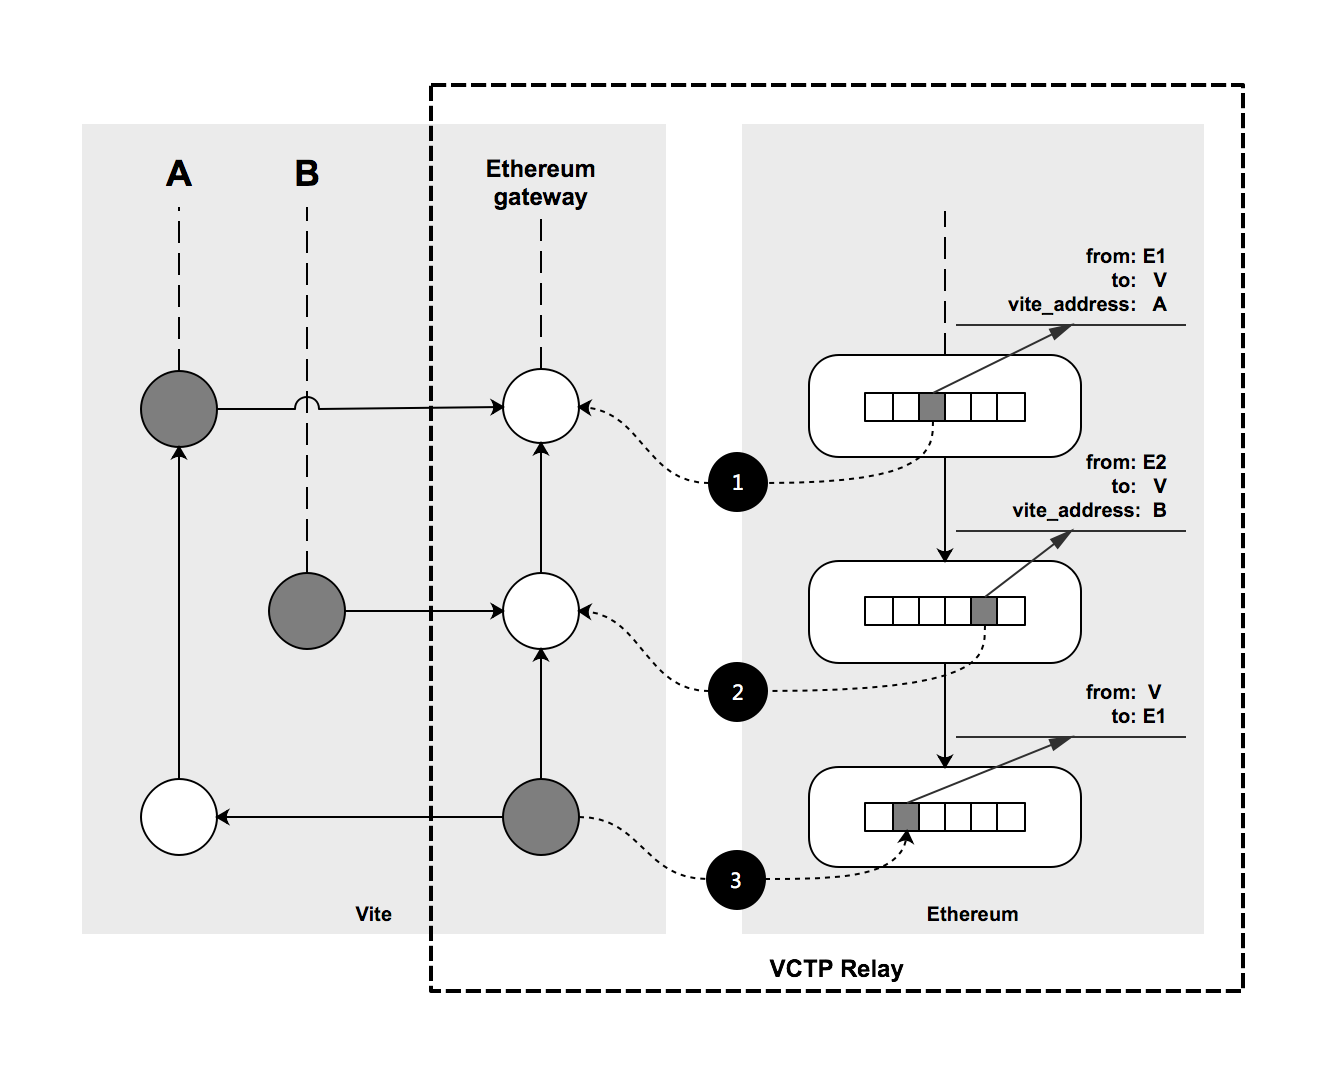
\includegraphics[width=\linewidth]{image/crosschain.png}
\caption{Cross Chain Protocol}
\end{figurehere}
\end{center}

The above picture is an example of the cross chain value transmission between the Vite and the Ethereum. When the Ethereum user $E1$ wants to transfer the token from the Ethereum to the Vite, it can send a transaction to the Vite gateway contract address $V$, while the user's address $A$ on the Vite is placed in the parameter. The balance of the transfer will be locked in the gateway contract account and become part of the ToT reserve. After listening to the transaction, the VCTP relay node generates a corresponding account sending transaction of Vite, sending the same amount of ToT to the user's account $A$ in the Vite. In the picture, \textcircled{1} and \textcircled{2} respectively indicate that $E1$ and $E2$ transfer to Vite account $A$ and $B$. It should be noted that if the user does not specify the Vite address when transferring, the contract will reject the transaction.

The reverse flow is shown in \textcircled{3}, When the user $A$ launches transfering from the Vite account to the Ethereum account, a transaction will be sent to the Vite gateway contract, transfers to a certain quantity of ToT, and specifies the reception address $E1$ of the Ethereum  in the transaction. The VCTP relay node will generate the corresponding response block on the Ethereum Gateway contract, and package a transaction of the Ethereum to the Vite gateway contract on the Ethereum. In the Ethereum , the Vite gateway contract will verify whether this transaction is initiated by a trusted VCTP relay, and then the same amount of \textit{ether} is transferred from the Vite gateway contract to the target account $E1$.

All cross chain relay nodes will monitor the target network, and they can verify whether each cross chain transaction is correct and reach consensus within the consensus group. But snapshot consensus group will not monitor the transaction of the target chain, nor will it verify whether the mapping between the two chains is correct. If the target network is rolled back or hard forked, the mapped transactions in the Vite system cannot be rolled back; similarly, if the cross chain transactions in the Vite are rolled back, the corresponding transaction of the target network can not be rolled back at the same time. Therefore, when doing cross - chain transactions, it is necessary to deal with transaction rollback in contract logic. At the same time, as described in the \ref{sec:consensus-prio} part, we need to set a \textit{delay} parameter for the cross chain Relay consensus group.

\subsection{Loopring Protocol}
Loopring protocol \cite{loopring} is an open protocol to build a decentralized asset trading network. Compared to other DEX solutions, the Loopring protocol is based on the multiparty loop matching, which provides a dual authorization technology to prevent preemptive transactions and is fully open.

We build the Loopring protocol into Vite, which is conducive to promoting the circulation of digital assets in Vite, so that the whole value system can be circulated. In this value system, users can issue their own digital assets, transfer assets outside the chain through VCTP, and use the Loopring protocol to achieve asset exchange. The whole process can be completed within the Vite system and is completely decentralized.

In Vite, Loopring Protocol Smart contract (LPSC) is a part of the Vite system. Asset transfer authorization and multi-party atomic protection are all supported in the Vite. The Loopring relay is still open to fully integrate with its own ecosystem.

Users can use \textit{vite} to pay for asset exchange transactions, so the earned token by miners of Looping who perform loop matching in the Vite platform is still \textit{vite}.


\section{Other Designs}
\subsection{Scheduling}
In the Ethereum, smart contracts are driven by transactions, and the execution of contracts can only be triggered by users initiating a transaction. In some applications, a timing scheduling function is needed to trigger the execution of a contract through a clock.

In Ethereum, this function is achieved through third party contracts.\footnote{\textit{Ethereum Alarm Clock} is a third party contract used to schedule the execution of other contracts, refer to \url{http://www.ethereum-alarm-clock.com/}}, performance and security are not guaranteed. In Vite, we add the timing scheduling function to the built in contract. The users can register their scheduling logic into the timed scheduling contract. The public consensus group will use the snapshot chain as a clock, and send the request transaction to the target contract according to the user defined scheduling logic.

There is a specialized \texttt{Timer} message in Solidity++. Users can set up their own scheduling logic in the contract code through \texttt{Timer.on}.

\subsection{Name Service}\label{sec:vns}
In Ethereum, the contract will generate an address to identify a contract when it is deployed. There are two problems in identifying contracts with addresses:
\begin{itemize}
	\item 	An address is an identifier with 20 bytes without meaning. It is unfriendly to users and inconvenient to use.
	\item 	Contracts and addresses are one-to-one. They cannot support contract redirection.
\end{itemize}

In order to solve these two problems, the developer of Ethereum has provided a third party contract ENS \footnote{\textit{Ethereum Name Service} is a third party contract used for name resoluton, refer to \url{https://ens.domains/}}. However, in the actual scenario, the use of naming services will be very frequent, and the use of third party contracts can not guarantee the global uniqueness of naming, so we will build a name service VNS (ViteName Service) in Vite.

Users can register a set of names which is easy to remember and resolve them to the actual address through VNS. Names are organized in the form of domain names, such as \textit{vite.myname.mycontract}. The top-level domain name will be retained by the system for specific purposes. For example, \textit{vite.xx} represents Vite address, and \textit{eth.xx} represents an Ethereum address. The second level domain name is open to all users.  Once the user owns the second level domain name, the subdomain can be expanded arbitrarily. The domain name owner can modify the address directed by the domain name at any time, so this function can be used for contract upgrading.

The length of the domain name is not restricted. In VNS, the hash of the domain name is actually stored. The target address can be a non Vite address of less than 256 bit, which can be used for cross chain interaction.

It should be noted that VNS is different from the smart contract Package specification EIP190\footnote{\textit{EIP190} Ethereum Smart Contract Packaging Specification,refer to \url{https://github.com/ethereum/EIPs/issues/190}} in Ethereum. VNS is a name resolution service, the name is established at runtime, and the resolution rules can be dynamically modified; and EIP190 is a package management specification, the namespace is static, and it is established at compile time.

\subsection{Contract Update}
The smart contract of Ethereum is immutable. Once deployed, it can not be modified. Even if there is a bug in the contract, it can not be updated. This is very unfriendly to developers and makes dApp's continuous iteration very difficult. Therefore, Vite needs to provide a scheme to support smart contract update.

In Vite, the process of contract updating includes:
\begin{itemize}
	\item[A.] Deploys a new version of the contract to inherit the status of the original contract.
	\item[B.] Points the name of the contract to the new address in VNS.
	\item[C.] Removes the old contract through the \textbf{SELFDESTRUCT} instruction
\end{itemize}

These three steps need to be completed at the same time, and the Vite protocol ensures the atomicity of the operation. Developers need to ensure that the old contract data are correctly processed in the new version contract.

It should be noted that the new contract will not inherit the address of the old contract. If quoted by the address, the transaction will still be sent to the old contract. This is because different versions of contracts are essentially two completely different contracts, whether they can be modified dynamically or not, depending on the semantics of contracts.

In Vite systems, smart contracts are actually divided into two types, the first one is the background of a dApp, and its business logic is described; and the second is a kind of contract that maps the real world. The previous one is equivalent to an application's background service, which needs to be continuously iterated through an upgrade; the latter is equivalent to a contract, and once it comes into effect, no modification can be made, otherwise it is a breach of contract. For such a contract that is not allowed to be modified, it can be decorated with keyword \textit{static} in Solidity++, for example:

\begin{verbatim}
pragma solidity++ ^0.1.0;

static contract Pledge {
    // the contract that will never change
}
\end{verbatim}

\subsection{Block Pruning}
In a ledger, any transaction is immutable, and users can only add new transactions to the ledger without altering or deleting historical transactions. Therefore, with the operation of the system, the ledgers will become bigger and bigger. If a new node who joining the network wants to restore the latest status, starting from the genesis block and redoing all the historical transactions. After running the system for a period of time, the space occupied by the account book and the time consumed for redoing transactions will become unacceptable. For the high throughput system of Vite, the rate of growth will be much higher than Bitcoin and Ethereum, so it is necessary to provide a technique for clipping the blocks in the ledgers.

Block clipping refers to the deletion of historical transactions that cannot be used in the ledgers, and does not affect the operation of the transactional state machine. So, which transactions can be safely deleted? It depends on which scenario the transaction will be used, including:


\begin{itemize}
\item \textbf{Recovery}.The primary role of a transaction is to recover status. Because in Vite, snapshot chain stores snapshot information of account status, nodes can recover state from a snapshot block. All transactions before \textit{lastTransaction} in the snapshot block can be tailored to state recovery.
\item \textbf{Verification of transactions}.To verify a new transaction, it needs to verify the exchange's previous transaction in the account chain, and if it is a response transaction, it also needs to verify the corresponding request transaction. Therefore, in the tailored accounting ledgers, at least one last transaction should be retained in each account chain. In addition, all open request transactions cannot be tailored because their hashes may be referenced by subsequent response transactions.
\item \textbf{Calculate quotas.}Whether a transaction meets the quota is calculated by judging the sliding average of the last 10 transaction resources, so at least the last 9 transactions need to be saved on each account chain.
\item \textbf{Inquire about history}. If the node needs to query the transaction history, the transaction involved in the query will not be tailored.
\end{itemize}

According to different usage scenarios, each node can choose several combinations from the above clipping strategy. It is important to note that clipping involves transactions in ledgers, while snapshot chains need to be kept intact. In addition, what is recorded in the snapshot chain is the hash of the contract state. When the account is clipped, the corresponding state of the snapshot needs to be kept intact.

In order to ensure the integrity of Vite data, we need to retain some "Full nodes" in the network to save all transaction data. Snapshot consensus group nodes are full nodes, and in addition, important users such as exchanges may also become full nodes.

\section{Governance}
For a decentralized application platform, an efficient governance system is essential for maintaining a healthy ecosystem. Efficiency and fairness should be considered when designing governance systems.

The governance system of Vite is divided into two parts: on-chain and off-chain. On-chain is a voting mechanism based on protocol, and off-chain is the iteration of the protocol itself.

On the voting mechanism, it is divided into two types: Global voting and local voting. The global voting is based on the \textit{vite} held by the user to calculate the rights as the voting weight. The global voting is mainly used for the election of the snapshot consensus group proxy node. The local vote is aimed at a contract. When the contract is deployed, a token is designated as the basis for voting. It can be used to elect the agent nodes of the consensus group in which the contract is located.

Besides the verification of transactions, the agent node of snapshot consensus group has the right to choose whether to upgrade the Vite system Incompatibility. The delegated consensus group proxy node has the right to decide whether to allow the contract to be upgraded so as to avoid potential risks arising from the escalation of contracts. The agent node is used to upgrade decision-making power on behalf of users in order to improve the efficiency of decision-making and avoid the failure of decision-making due to insufficient participation in voting. These proxy nodes themselves are also restricted by consensus protocol. Only if most \footnote{according to DPoS protocol, the valid majority is 2/3 of total agent nodes.} agent nodes are passed, will the upgrade take effect. If these agents do not fulfill their decision-making power according to the user's expectations, users can also cancel their proxy qualification by voting.

The governance of off-chain is realized by the community. Any Vite community participant can propose an improvement plan for the Vite protocol itself or related systems, which is called VEP (Vite Enhancement Proposal). VEP can be widely discussed in the community and whether to implement the solution is decided by Vite ecological participants. Whether the protocol will be upgraded for the implementation of a VEP will be ultimately decided by the agent node. Of course, when the differences are large, you can also start a round of voting on the chain to collect a wide range of user opinions, and the proxy node will decide whether to upgrade according to the result of the vote.

Although some Vite participants may not have enough \textit{vite} tokens to vote for their opinions. But they can freely submit VEP and fully express their views. The users who have the right to vote must take full account of the health of the whole ecology for their own Vite rights, and therefore take the views of all the ecological participants seriously.


\section{Tasks in future}
Transaction verification on snapshot chains is a major performance bottleneck of the system. Because Vite adopts asynchronous design and DAG account structure, transaction validation can be executed in parallel. However, due to the dependence between the transactions of different accounts, the degree of parallelism will be greatly restricted. How to improve the parallelism of transaction verification or adopt a distributed verification strategy will be an important direction for future optimization.

Some shortcomings exist in the current HDPoS consensus algorithm as well. It is also an optimization direction to improve the consensus algorithm, or to be compatible with more consensus algorithms in the delegated consensus group.

In addition, the optimization of virtual machine is also very important for reducing system delay and improving system throughput. Because of the simple design of EVM and the simplification of the instruction set, it may be necessary to design a more powerful virtual machine in the future and define a smart contract programming language with more ability to describe and less security vulnerabilities.

Finally, besides the Vite core agreement, the construction of ancillary facilities supporting ecological development is also an important topic. In addition to SDK support for dApp developers, there is much work to do in dApp foreground ecosystem construction. For example, you can build a dApplet engine based on HTML5 in the mobile wallet application of Vite, allowing developers to develop and publish dApp at low cost.

\section{Summary}
Compared with other similar projects, the characteristics of Vite include:

\begin{itemize}
	\item \textbf{High throughput}.Vite uses the DAG ledger structure, the orthogonal transaction can be written in parallel to the book; in addition, multiple conconsensus groups do not depend on each other in the HDPoS consensus algorithm, and can work in parallel; the most important thing is that the Vite's inter contract communication is based on the asynchronous model of the message. All these are helpful to improve the throughput of the system.
	\item \textbf{Low delay}.Vite uses the HDPoS consensus algorithm to collaborate to complete the rotation production block through the proxy node, without the need to calculate PoW, the block interval can be reduced to 1 second, which is beneficial to reduce the delay of transaction confirmation.
	\item \textbf{Scalability}.In order to meet the scalability requirements, Vite makes a single degree of freedom limit on the transaction, grouping the transactions in the account according to the account dimension, allowing the block production of different accounts to be completed by different nodes, and to remove the ACID semantics of the cross contract calls to BASE semantics based on the message. In this way, nodes no longer need to save all the state of the world, and the data are saved in the entire distributed network in sharding mode
	\item \textbf{Usability}.The improvements of Vite's usability include providing standard library support in Solidity++, dedicated to processing message syntax, timing scheduling of contract, VNS naming services, support of contract upgrading, and so on.
	\item \textbf{Value circulation}.Vite supports digital asset issuance, cross chain value transfer, token exchange based on Loopring protocol, and so on, forming a complete value system. From the user's point of view, Vite is a fully functional decentralized exchange.
	\item \textbf{Economy}.Because Vite adopts quota based resource allocation model, lightweight users who do not trade frequently do not have to pay high fees or gas charges. Users can choose a variety of ways to change the calculation. Extra quota can also be transferred to other users through quota leasing agreement to improve the efficiency of system resource utilization.
\end{itemize}
\section{Thanks}
Sincerely, we would like to thank our consultants for their guidance and assistance to this article. Especially We would like to appreciate the contribution of Loopring team and Loopring community to this project. 

\end{multicols}

\bibliography{vite}
\bibliographystyle{unsrt}


\begin{appendices}

\section{EVM Instruction set\label{app:evm-instruction-set}}
\subsubsection{0s: Stop and algebraic operation instruction set}
\begin{tabu}{l l l l l l} \savetabu{opcodes}
\toprule

\textbf{No.} & \textbf{Words} & \textbf{POP} & \textbf{PUSH} & \textbf{Semantics in EVM} & \textbf{Semantics in Vite}  \vspace{5pt} \\
0x00 & {\small STOP} & 0 & 0 & Stop to Excute. &  Sanme semantics\\
\midrule
0x01 & {\small ADD} & 2 & 1 & Add two operands. & Same semantics\\
\midrule
0x02 & {\small MUL} & 2 & 1 & Multiplying two operands. & Same semantics\\
\midrule
0x03 & {\small SUB} & 2 & 1 & Subtracting two operands. & Same semantics\\
\midrule
0x04 & {\small DIV} & 2 & 1 & Divide two operands & Same semantics\\
&&&&  If the divisor is 0 \\ 
&&&&  then returns 0 \\

\midrule
0x05 & {\small SDIV} & 2 & 1 & Divided with symbol. & Same semantics\\
\midrule
0x06 & {\small MOD} & 2 & 1 & Modulus Operation. & Same semantics\\
\midrule
0x07 & {\small SMOD} & 2 & 1 & Modulus with symbol. & Same semantics\\
\midrule
0x08 & {\small ADDMOD} & 3 & 1 &Add the first two & Same semantics\\
&&&& operands and module with 3rd \\

\midrule
0x09 & {\small MULMOD} & 3 & 1 & Mmultiply the first two  & Same semantics\\
&&&& operands and module with 3rd \\
\midrule
0x0a & {\small EXP} & 2 & 1 & The square of two operands. & Same semantics\\
\midrule
0x0b & {\small SIGNEXTEND} & 2 & 1 & Symbol extension. & Same semantics\\
\midrule
\end{tabu}

\subsubsection{10s: Comparison and bit operation instruction set}
\begin{tabu}{\usetabu{opcodes}}
\toprule
\textbf{No.} & \textbf{Words} & \textbf{POP} & \textbf{PUSH} & \textbf{Semantics in EVM} & \textbf{Semantics in Vite}  \vspace{5pt} \\

0x10 & {\small LT} & 2 & 1 & less than. &  Same semantics\\
\midrule
0x11 & {\small GT} & 2 & 1 & greater than. &  Same semantics\\
\midrule
0x12 & {\small SLT} & 2 & 1 & less than with symbol. &  Same semantics\\
\midrule
0x13 & {\small SGT} & 2 & 1 & greater than with symbol. &  Same semantics\\
\midrule
0x14 & {\small EQ} & 2 & 1 & equal to. &  Same semantics\\
\midrule
0x15 & {\small ISZERO} & 1 & 1 & if it is 0. &  Same semantics\\
\midrule
0x16 & {\small AND} & 2 & 1 & And by bit. &  Same semantics\\
\midrule
0x17 & {\small OR} & 2 & 1 & Or by bit. &  Same semantics\\
\midrule
0x18 & {\small XOR} & 2 & 1 & Xor by bit. &  Same semantics\\
\midrule
0x19 & {\small NOT} & 1 & 1 & Nor by bit. &  Same semantics\\
\midrule
0x1a & {\small BYTE} & 2 & 1 & Take one of byte  &  Same semantics\\
&&&& from the second operands.\\

\bottomrule
\end{tabu}

\subsubsection{20s: SHA3 instruction set}
\begin{tabu}{\usetabu{opcodes}}
\toprule
\textbf{No.} & \textbf{Words} & \textbf{PoP} & \textbf{PUSH} & \textbf{Semantics in EVM} & \textbf{Semantics in Vite} \vspace{5pt} \\
0x20 & {\small SHA3} & 2 & 1 & Calculate Keccak-256 hash. &  Same semantics\\

\bottomrule
\end{tabu}

\subsubsection{30s: Environmental information instruction set}
\begin{tabu}{\usetabu{opcodes}}
\toprule
\textbf{No.} & \textbf{Words} & \textbf{POP} & \textbf{PUSH} & \textbf{Semantics in EVM} & \textbf{Semantics in Vite}  \vspace{5pt} \\

0x30 & {\small ADDRESS} & 0 & 1 & Obtain address . &  Same semantics\\
&&&& of current account \\
\midrule
0x31 & {\small BALANCE} & 1 & 1 &  Obtain the balance &  Same semantics.\\
&&&&  of an account.\\
&&&&& returned is the \\
&&&&&  \textit{vite} balance of account\\
\midrule
0x32 & {\small ORIGIN} & 0 & 1 & Obtain the sender   & Different samantics\\
&&&& addresss of original transaction\\
&&&&& return 0 forever\\
&&&&& Vite doesn't maintain \\
&&&&& the causal relationship \\
&&&&& between internal transaction \\
&&&&& and user transaction.\\
\midrule
0x33 & {\small CALLER} & 0 & 1 & Obtain the address  & Same semantics.\\
&&&& of direct caller.\\
\midrule
0x34 & {\small CALLVALUE} & 0 & 1 & Obtain the transferred  & Same semantics\\
&&&& amount in called transaction.\\
\midrule
0x35 & {\small CALLDATALOAD} & 1 & 1 & Obtain the parameter & Same semantics\\
&&&&  in this calling\\
\midrule
0x36 & {\small CALLDATASIZE} & 0 & 1 & Obtain size of  & Same semantics\\
&&&& parameter \\
&&&& data in this calling.\\
\midrule
0x37 & {\small CALLDATACOPY} & 3 & 0 & Copy called parameter & Same semantics \\
&&&&  data into memory.\\
\midrule
0x38 & {\small CODESIZE} & 0 & 1 & Obtain the size  & Same semantics\\
&&&& of the running code in \\
&&&& current environment.\\
\midrule
0x39 & {\small CODECOPY} & 3 & 0 & Copy the running  & Same semantics\\
&&&& code in current environment \\
&&&& into memory.\\
\midrule
0x3a & {\small GASPRICE} & 0 & 1 & Obtain the gas . & Different samantics\\
&&&& price in current enviroment\\
&&&&& ,return 0 forever.\\
\midrule
0x3b & {\small EXTCODESIZE} & 1 & 1 & Obtain the code  & Same semantics \\
&&&& size of an account.\\
\midrule
0x3c & {\small EXTCODECOPY} & 4 & 0 & Copy the code of. & Same semantics\\
&&&&  an account into memory\\
\midrule
0x3d & {\small RETURNDATASIZE} & 0 & 1 & Obtain data size  & Same semantics\\
&&&& of returned from \\
&&&& previous calling.\\
\midrule
0x3e & {\small RETURNDATACOPY} & 3 & 0 & Copy the returned  &  Same semantics\\
&&&& data calling \\
&&&& previously into memory\\
&&&& into memory.\\
\bottomrule
\end{tabu}

\subsubsection{40s: Block info instructions set}
\begin{tabu}{\usetabu{opcodes}}
\toprule
\textbf{No.} & \textbf{Words} & \textbf{POP} & \textbf{PUSH} & \textbf{Semantics in EVM} & \textbf{Semantics in Vite}  \vspace{5pt} \\

0x40 & {\small BLOCKHASH} & 1 & 1 & Obtain hash of a block. & Different semantic.\\
&&&&& return Hash of  \\
&&&&& corresponing snapshot block.\\
\midrule
0x41 & {\small COINBASE} & 0 & 1 & Obtain the address. & Different semantic.\\
&&&&  of miner beneficiary \\
&&&& in current block\\
&&&&& return 0 forever. \\
\midrule
0x42 & {\small TIMESTAMP} & 0 & 1 & Return timestamp  & Different semantic.\\
&&&& of current block.\\
&&&&& return 0 forever. \\
\midrule
0x43 & {\small NUMBER} & 0 & 1 & Return the number  & Different semantic.\\
&&&& or current block.\\
&&&&& Return the number of \\
&&&&& responding transaction \\
&&&&& block in account chain \\
\midrule
0x44 & {\small DIFFICULTY} & 0 & 1 & Return the difficulty & Different semantic.\\
&&&&  of the block.\\
&&&&& return 0 forever. \\
\midrule
0x45 & {\small GASLIMIT} & 0 & 1 & Return the gas. & Different semantic.\\
&&&&  limitation of the block\\
&&&&& return 0 forever. \\
\bottomrule
\end{tabu}

\subsubsection{50s: Stach、Memory、Storege、Control stream operation instruction set}
\begin{tabu}{\usetabu{opcodes}}
\toprule
\textbf{No.} & \textbf{Words} & \textbf{POP} & \textbf{PUSH} & \textbf{Semantics in EVM} & \textbf{Semantics in Vite}  \vspace{5pt} \\

0x50 & {\small POP} & 1 & 0 & Pop one data & Same semantics\\
&&&&  from top of stack.\\
\midrule
0x51 & {\small MLOAD} & 1 & 1 & load a word from memory. & Same semantics\\

\midrule
0x52 & {\small MSTORE} & 2 & 0 & Save a word to memory & Same semantics\\

\midrule
0x53 & {\small MSTORE8} & 2 & 0 & Save a byte to memory. & Same semantics\\

\midrule
0x54 & {\small SLOAD} & 1 & 1 & Load a word from storage. & Same semantics\\

\midrule
0x55 & {\small SSTORE} & 2 & 0 & Save a word into storage. & Same semantics\\
\midrule
0x56 & {\small JUMP} & 1 & 0 & Jump instructions. & Same semantics\\
\midrule
0x57 & {\small JUMPI} & 2 & 0 & Jump instructions with condition. & Same semantics\\
\midrule
0x58 & {\small PC} & 0 & 1 & Obtain program counter's value. & Same semantics\\
\midrule
0x59 & {\small MSIZE} & 0 & 1 & Obtain size of memory. & Same semantics\\
\midrule
0x5a & {\small GAS} & 0 & 1 & Obtain available gas . &  Different semantic.\\
&&&&& return 0 forever. \\
\midrule
0x5b & {\small JUMPDEST} & 0 & 0 & Mark a destination of jumping . & Same semantics\\
\bottomrule
\end{tabu}

\subsubsection{60s and 70s: Stack operation instructions}
\begin{tabu}{\usetabu{opcodes}}
\toprule
\textbf{No.} & \textbf{Words} & \textbf{POP} & \textbf{PUSH} & \textbf{Semantics in EVM} & \textbf{Semantics in Vite}  \vspace{5pt} \\

0x60 & {\small PUSH1} & 0 & 1 & Push one byte object. & Same semantics\\
&&&&  into top of stack\\

\midrule
0x61 & {\small PUSH2} & 0 & 1 & Push two bytes object  & Same semantics \\
&&&& into top of stack.\\

\midrule
\multicolumn{1}{c}{\vdots} & \multicolumn{1}{c}{\vdots} & \vdots & \vdots & \multicolumn{1}{c}{\vdots} \\
\midrule
0x7f & {\small PUSH32} & 0 & 1 & Push 32 bytes object   & Same semantics \\
&&&& (whole word) into \\
&&&& top of stack\\

\bottomrule
\end{tabu}

\subsubsection{80s: Duplication operation instructions}
\begin{tabu}{\usetabu{opcodes}}
\toprule
\textbf{No.} & \textbf{Words} & \textbf{POP} & \textbf{PUSH} & \textbf{Semantics in EVM} & \textbf{Semantics in Vite}  \vspace{5pt} \\

0x80 & {\small DUP1} & 1 & 2 & Duplicate 1st object and & Same semantics \\
&&&&  push it into top of stack.\\

\midrule
0x81 & {\small DUP2} & 2 & 3 & Duplicate 2nd object  . & Same semantics \\
&&&& and push it into top of stack.\\

\midrule
\multicolumn{1}{c}{\vdots} & \multicolumn{1}{c}{\vdots} & \vdots & \vdots & \multicolumn{1}{c}{\vdots} \\
\midrule
0x8f & {\small DUP16} & 16 & 17 & Duplicate 16th object  & Same semantics \\
&&&&  and push it into top of stack.\\

\bottomrule
\end{tabu}

\subsubsection{90s: Swap operation instructions}
\begin{tabu}{\usetabu{opcodes}}
\toprule
\textbf{No.} & \textbf{Words} & \textbf{POP} & \textbf{PUSH} & \textbf{Semantics in EVM} & \textbf{Semantics in Vite}  \vspace{5pt} \\

0x90 & {\small SWAP1} & 2 & 2 & Swap 1st and 2nd  & Same semantics \\
&&&& object in stack.\\

\midrule
0x91 & {\small SWAP2} & 3 & 3 & Swap 1st and 3rd  & Same semantics \\
&&&& object in stack.\\

\midrule
\multicolumn{1}{c}{\vdots} & \multicolumn{1}{c}{\vdots} & \vdots & \vdots & \multicolumn{1}{c}{\vdots} \\
\midrule
0x9f & {\small SWAP16} & 17 & 17 & Swap 1st and 17th  & Same semantics \\
&&&& object in stack.\\

\bottomrule
\end{tabu}

\subsubsection{a0s: Log operation instructions}
\begin{tabu}{\usetabu{opcodes}}
\toprule
\textbf{No.} & \textbf{Words} & \textbf{POP} & \textbf{PUSH} & \textbf{Semantics in EVM} & \textbf{Semantics in Vite}  \vspace{5pt} \\

0xa0 & {\small LOG0} & 2 & 0 & Extend log record, & Same semantics\\
&&&& no scheme.\\

\midrule
0xa1 & {\small LOG1} & 3 & 0 & Extend log record,. & Same semantics \\
&&&& 1 scheme\\

\midrule
\multicolumn{1}{c}{\vdots} & \multicolumn{1}{c}{\vdots} & \vdots & \vdots & \multicolumn{1}{c}{\vdots} \\
\midrule
0xa4 & {\small LOG4} & 6 & 0 & Extend log record,. & Same semantics\\
&&&& 4 schemes\\ 

\bottomrule
\end{tabu}

\subsubsection{f0s: System operation instructions}
\begin{tabu}{\usetabu{opcodes}}
\toprule
\textbf{No.} & \textbf{Words} & \textbf{POP} & \textbf{PUSH} & \textbf{Semantics in EVM} & \textbf{Semantics in Vite}  \vspace{5pt} \\

0xf0 & {\small CREATE} & 3 & 1 & Create a new contract. & Same semantics \\

\midrule
0xf1 & {\small CALL} & 7 & 1 & Call another contract. & Different semantic. \\
&&&&& indicate sending \\
&&&&& a message to an account\\
&&&&& The returned vale is 0 forever.\\

\midrule
0xf2 & {\small CALLCODE} & 7 & 1 & Call the code of  & Same semantics \\
&&&& another contract\\
&&&& Change the status of account. \\

\midrule
0xf3 & {\small RETURN} & 2 & 0 & Stop execution  & Same semantics \\
&&&& and return value.\\

\midrule
0xf4 & {\small DELEGATECALL} & 6 & 1 & Call the code of  & Same semantics \\
&&&& another contract, change\\
&&&& contract, change current  \\
&&&& account status keep \\
&&&& original transaction info.\\

\midrule
0xfa & {\small STATICCALL} & 6 & 1 & Call another contract, & Different semantic. \\
&&&&  not allow to change status.\\
&&&&& represents to sending\\
&&&&& message to a contract,\\
&&&&& don't change status of \\
&&&&& target contract.\\
&&&&& return 0 forever.needed result \\
&&&&& Sending another message through \\
&&&&& target contract and return. \\

\midrule
0xfd & {\small REVERT} & 2 & 0 & Stop execution and . & Same semantics \\
&&&& recover status and return value \\
&&&&& no semantics of returning left gas.\\

\midrule
0xfe & {\small INVALID} & $\varnothing$ & $\varnothing$ & invalid instructions. & Same semantics \\
\midrule

0xff & {\small SELFDESTRUCT} & 1 & 0 & Stop execution, & Same semantics \\
&&&& set the contract \\
&&&&  as waiting for deleting\\
&&&& return all balance. \\
\bottomrule
\end{tabu}


\end{appendices}
\end{document}
